
\input{"C:/Users/spileggi/Google Drive/STAT 330/Lectures/SlideStyle.tex"}




\title[Lecture 15]{PROC TABULATE}
\author[Pileggi]{Shannon Pileggi}

\institute[STAT 330]{STAT 330}

\date{}


\begin{document}

\begin{frame}
\titlepage
\end{frame}

\begin{frame}
\frametitle{OUTLINE\qquad\qquad\qquad} \tableofcontents[hideallsubsections]
\end{frame}


%===========================================================================================================================
\section[Overview]{Overview}
%===========================================================================================================================
\subsection{}
\begin{frame}
\ft{Overview}
\hspace*{-0.3in}
\begin{tabular}{|l|ccc|ccccc|}
\hline
\ttt{PROC}    & Detail  & Summary & Control & N        & sum    & mean & std & \% \\
\hline
\hline
\ttt{PRINT}   &  \gc    &    \rx  & \gc &  \gc    &    \gc  & \rx & \rx      &  \rx   \\
\ttt{MEANS}   &  \rx    &    \gc  & \rx &  \gc    &    \gc  & \gc & \gc      &  \rx    \\
\ttt{FREQ}    &  \rx    &    \gc  & \rx &  \gc    &    \rx  & \rx & \rx      &  \gc \\
\hline
\ttt{REPORT}  &  \gc    &    \gc  & \gc &  \gc    &    \gc  & \gc & \gc      &  \gc \\
\ttt{TABULATE}&  \rx    &    \gc  & \gc &  \gc    &    \gc  & \gc & \gc      &  \gc \\
\ttt{SQL}     &  \gc    &    \gc  & \rx &  \gc    &    \gc  & \gc & \gc      &  \gc  \\
\hline
\end{tabular}
\begin{itemize}
\item Detail: display a row for each observation
\item Summary: display a row for a group of observations
\item Control: many layout/format/display options in output
\item \ttt{SQL}: can additionally combine and sort data
\end{itemize}
\end{frame}

\begin{frame}
\ft{Patents data}
\bi
\item number of utility patent (``patents for inventions'') grants from 2011, by county
\item demographic variables from the American Community Survey
\bi
\item some variables may be missing for smaller counties
\ei
\item San Jose, CA (Santa Clara County)
\bi
\item $3^{rd}$ largest city in CA, $10^{th}$ largest city in US
\item leads all US cities in generating patents
\ei
\ei
\oyo Explore the \ttt{patents} data in SAS.
\end{frame}

\begin{frame}
\ft{Goal}
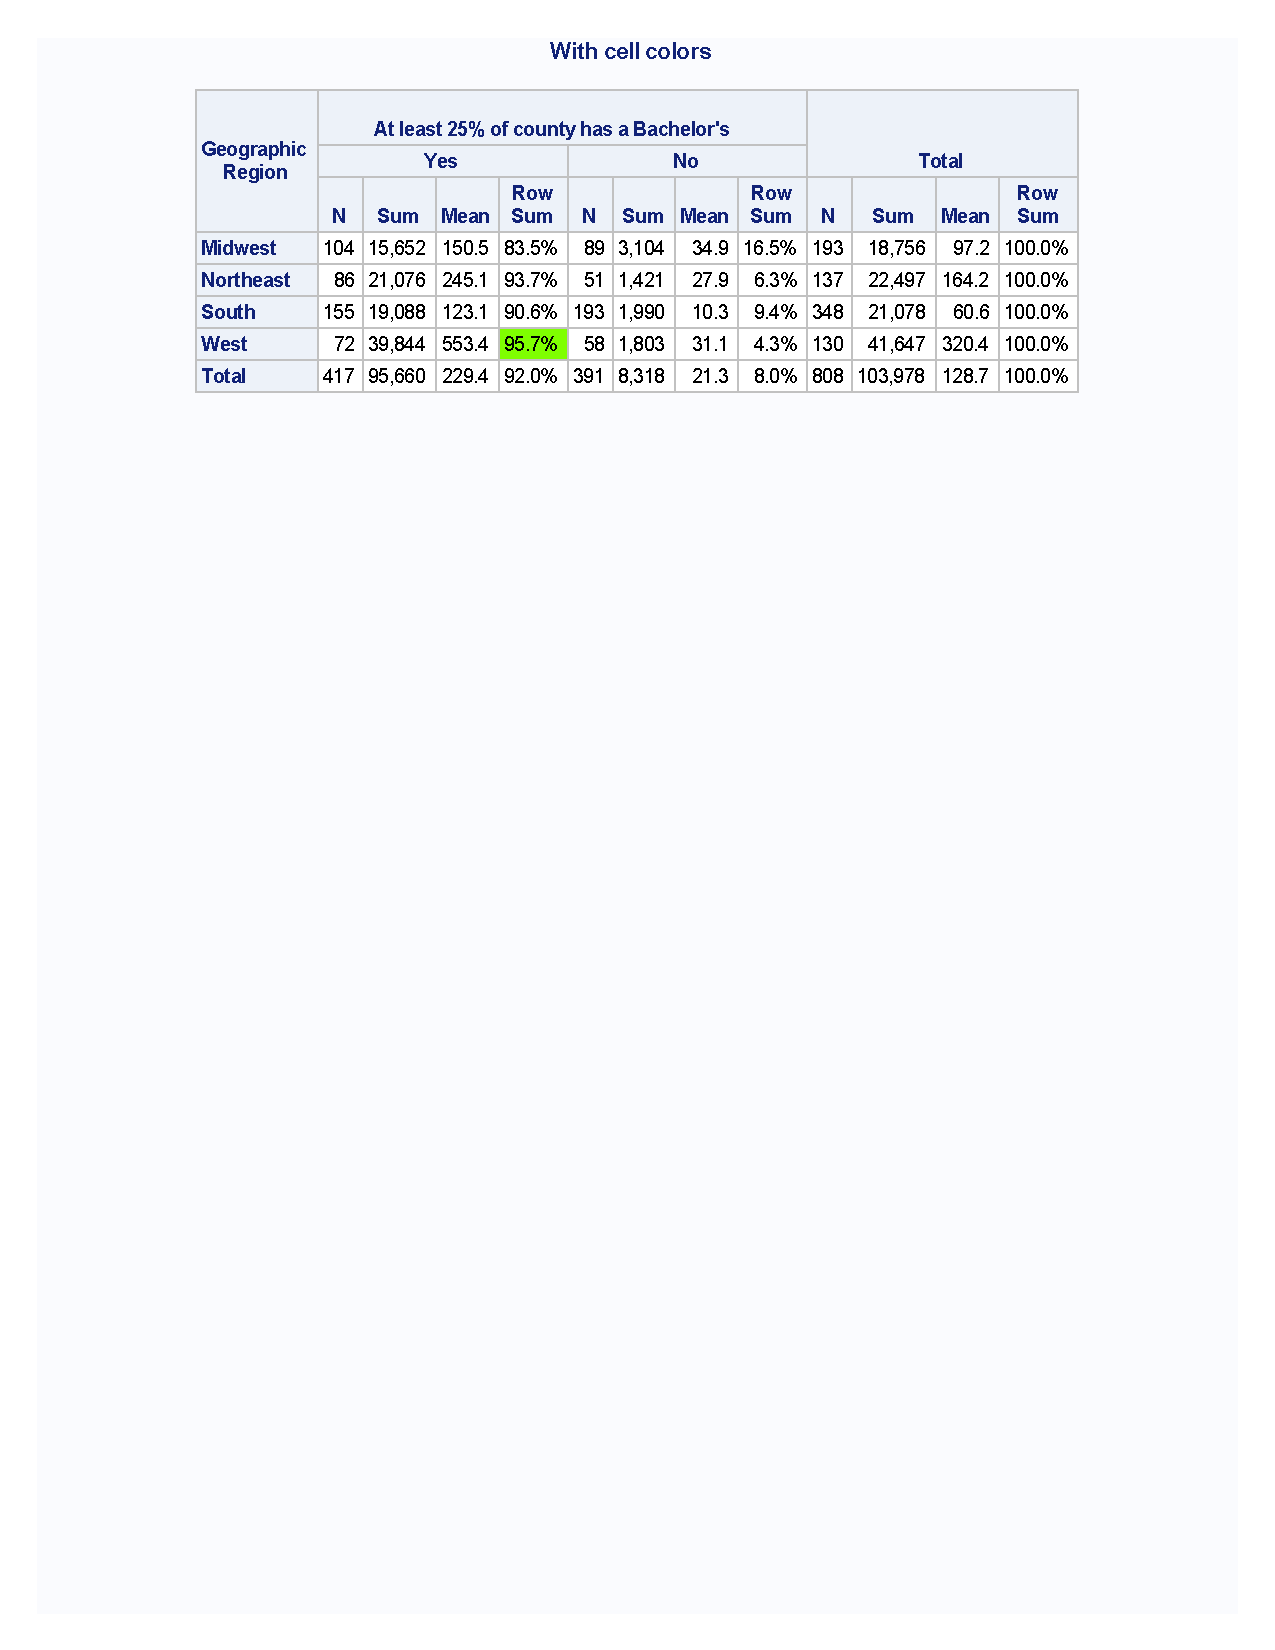
\includegraphics[trim={2cm 21cm 2cm 1.5cm},clip,width=1.0\textwidth]{L15_highlight.pdf}
\bi
\item Region along rows, education status along columns
\item Row and column totals
\item Various statistics reported, formatted values in cells
\item Highlighted cell: in the west region, 95.7\% of all patents come from counties with higher education levels
\item Style modified and exported to a pdf
\ei
\end{frame}

%===========================================================================================================================
\section[Structure]{Structure}
%===========================================================================================================================
\subsection{}
\begin{frame}
\tableofcontents[currentsection, hideallsubsections]
\end{frame}

\begin{frame}[fragile]
\ft{Syntax}
\bmp{.65\textwidth}
\begin{code}{.}
PROC TABULATE DATA = \emph{dataset} ;
   CLASS \emph{catvar1} \emph{catvar2...}  ;
   VAR   \emph{quantvar1} \emph{quantvar2...} ;
   TABLE \emph{page-var}, \emph{row-var}, \emph{col-var};
RUN;
\end{code}
\emp
\bmp{0.05\textwidth} \hspace{0.05in} \emp
\bmp{0.30\textwidth}
Each variable listed in \ttt{TABLE} statement \ttb{must} also be listed in either \ttt{CLASS} or \ttt{VAR}.
\emp
\vskip10pt
\bmp{0.3\textwidth}\hspace{0.05in} \emp
\bmp{0.7\textwidth}
\bi
\item[\fbox{\ttt{TABLE} \emph{var1};}] one-dimensional table with \emph{var1} on columns
\item[\fbox{\ttt{TABLE} \emph{var2}, \emph{var1};}] two-dimensional table with \emph{var2} on rows, \emph{var1} on columns
\item[\fbox{\ttt{TABLE} \emph{var3}, \emph{var2}, \emph{var1};}] three-dimensional table with \underline{page by} \emph{var3}, \emph{var2} on rows, \emph{var1} on columns
\ei
\emp
\end{frame}

%\begin{frame}
%\ft{Practice}
%\oyo Produce a
%\begin{enumerate}
%\item One-dimensional table with \ttt{edu25} on the columns
%\item Two-dimensional table with \ttt{edu25} on the columns and \ttt{region} on the rows
%\item Three dimensional table with page by \ttt{unemp10}, \ttt{edu25} on the columns, and \ttt{region} on the rows
%\end{enumerate}
%\bi
%\item[]
%\item The default statistic produced is is the number of observations ($N$) in each category.
%\item A three-dimensional table in \ttt{PROC TABULATE} is like using a \ttt{BY} statement in other \ttt{PROCs}
%\ei
%\end{frame}

\begin{frame}[fragile]
%\ft{One- and two-dimensional tables}
\hspace*{-0.3in}
\bmp{.52\textwidth}
One-dimensional table
\begin{itemize}
\item columns = \ttt{edu25}
\item[]
\end{itemize}
\begin{code}{.}
PROC TABULATE DATA = patents ;
   CLASS edu25 ;
   TABLE edu25 ;
RUN ;
\end{code}
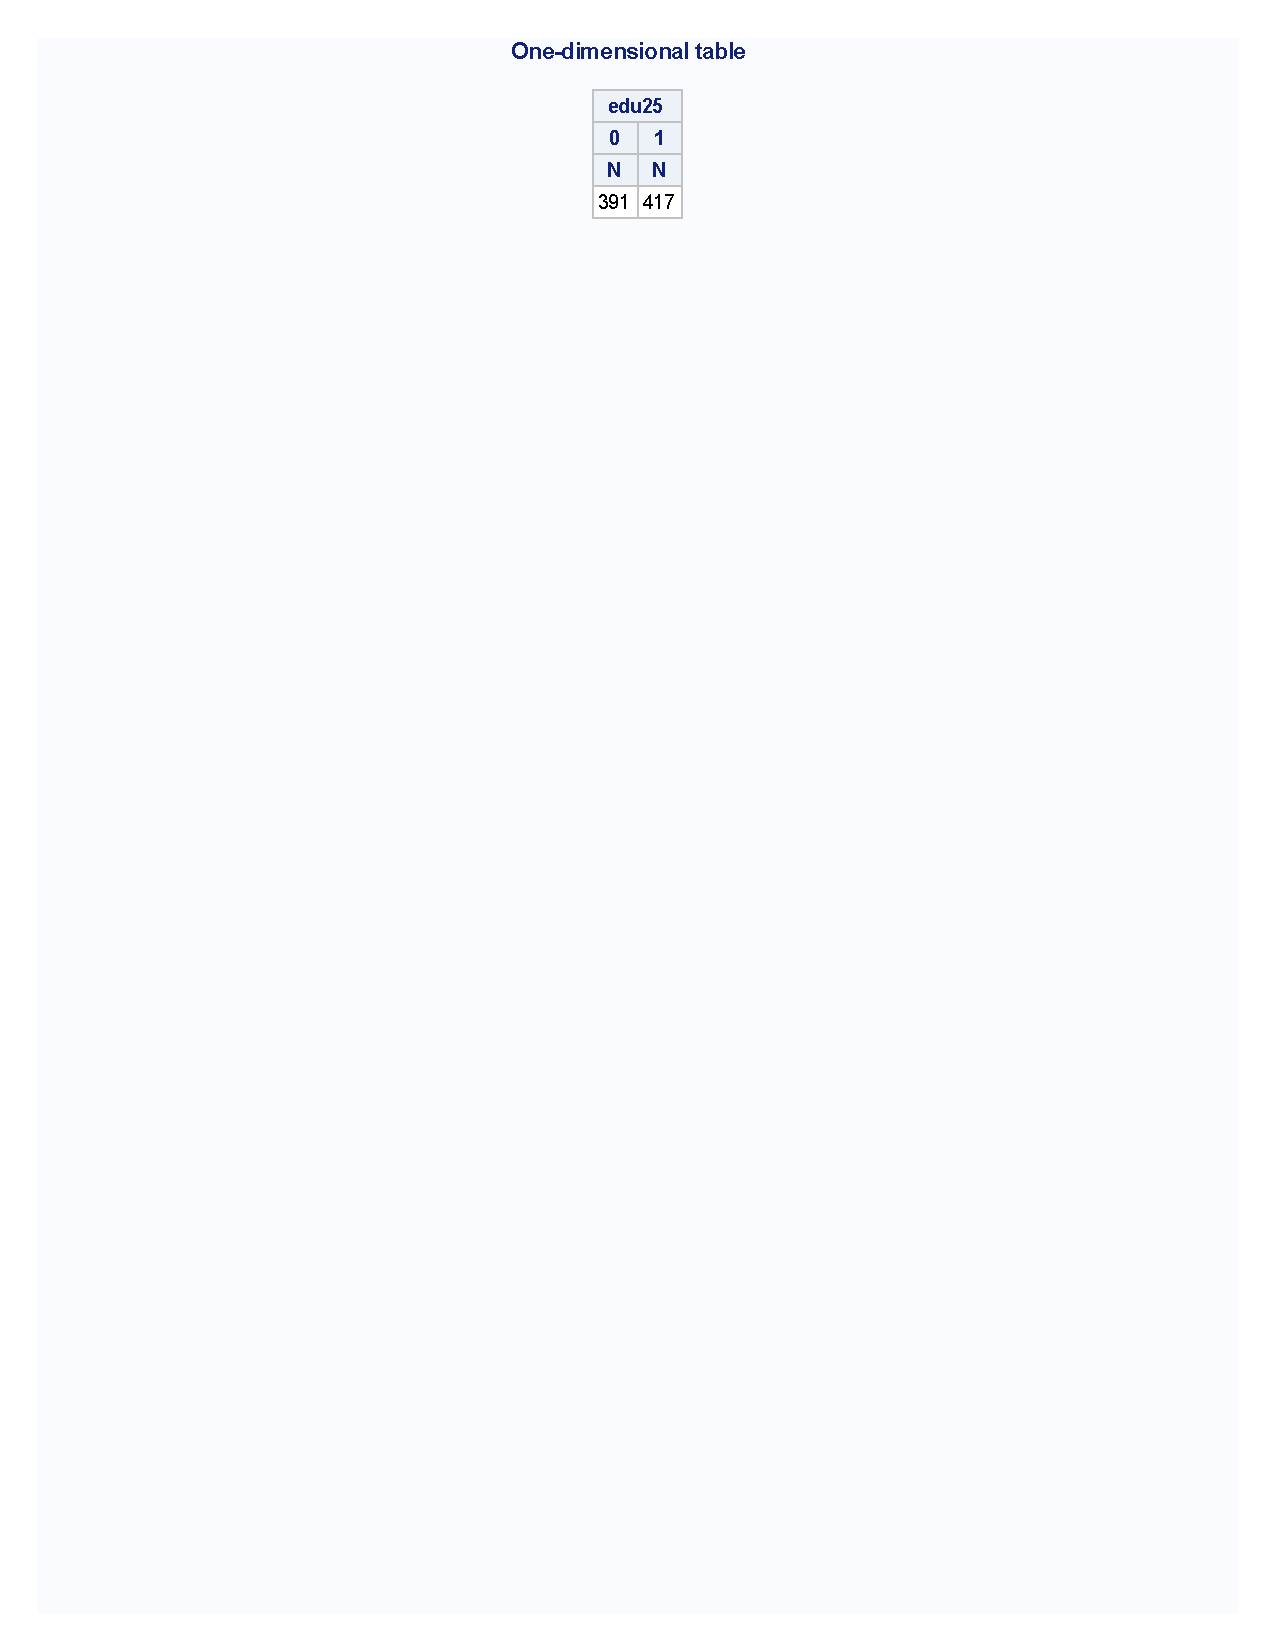
\includegraphics[trim={6.5cm 22cm 6.5cm 1.5cm},clip,width=1.0\textwidth]{L15_1dtable.pdf}
\emp
\blankcolumn
\bmp{.52\textwidth}
Two-dimensional table
\begin{itemize}
\item columns = \ttt{edu25}
\item rows = \ttt{region}
\end{itemize}
\begin{code}{.}
PROC TABULATE DATA = patents ;
   CLASS edu25 region ;
   TABLE region, edu25 ;
RUN ;
\end{code}
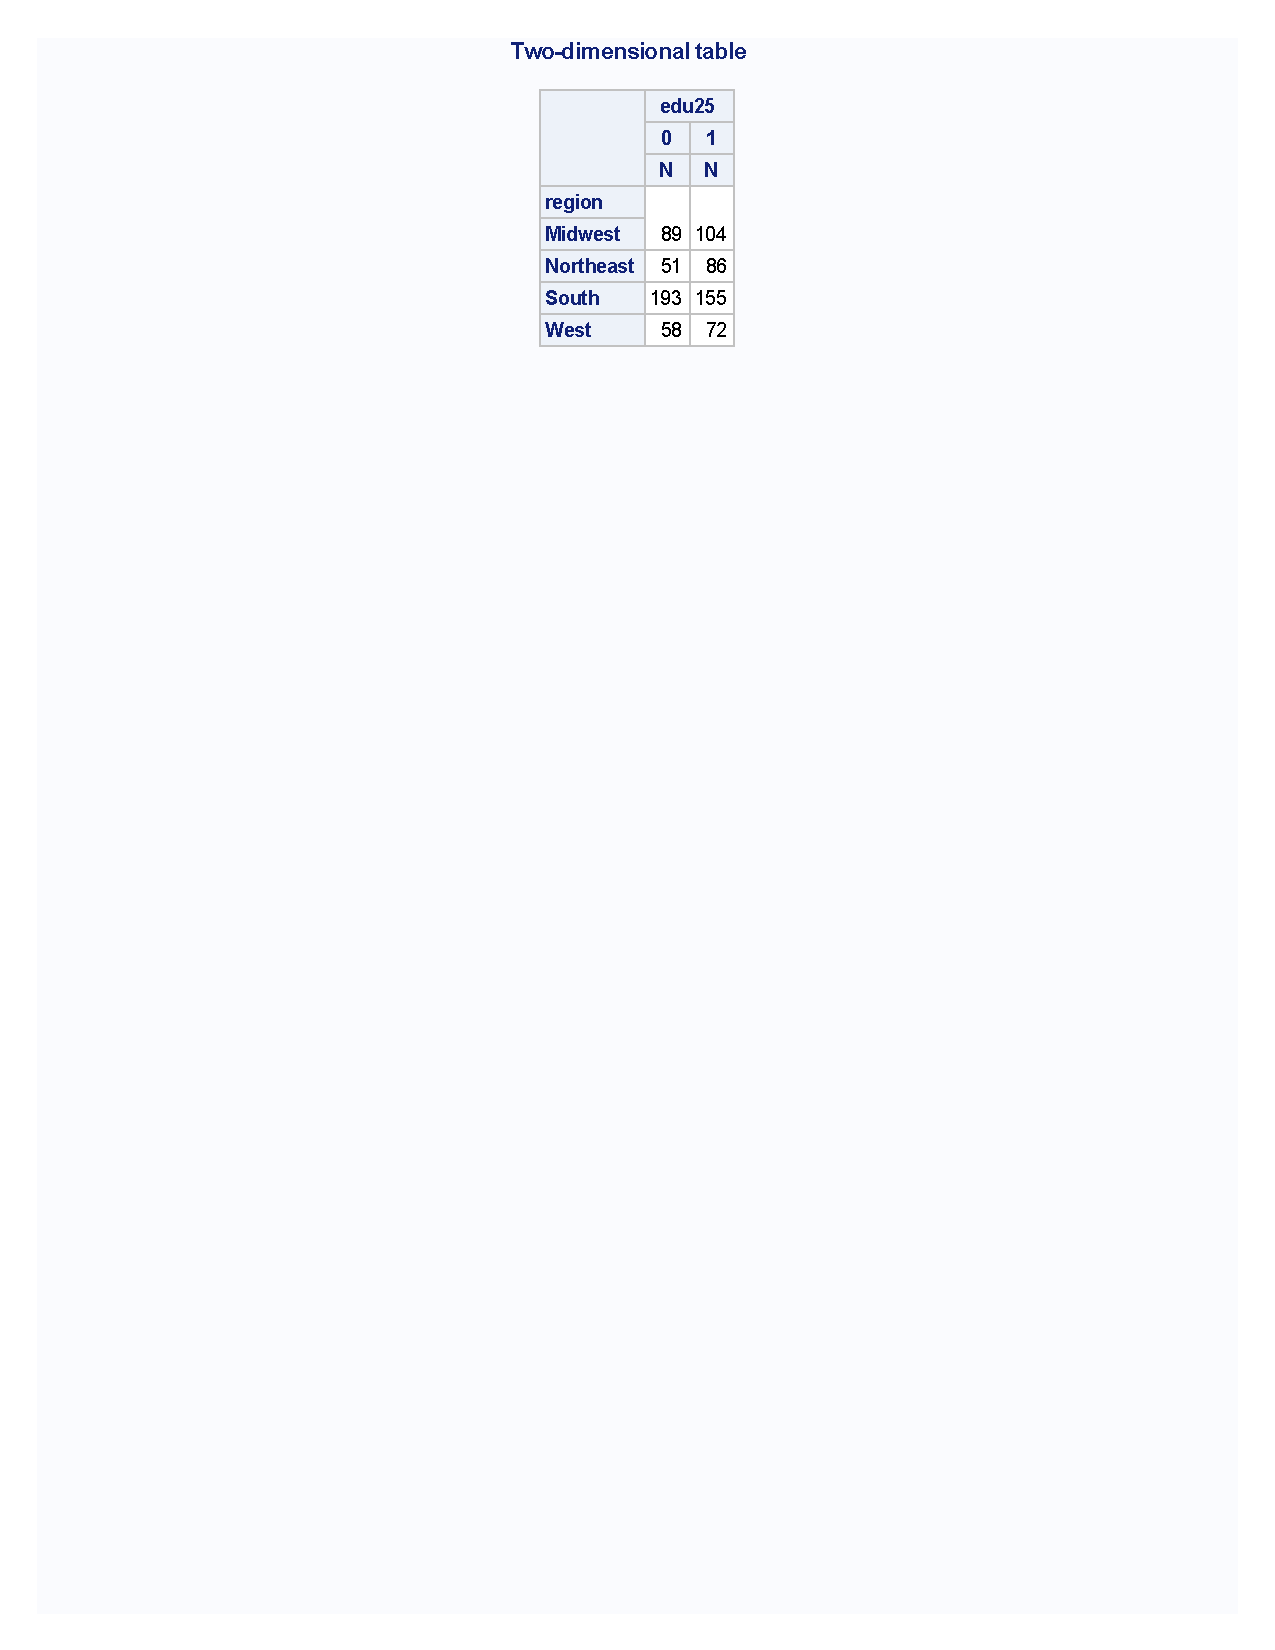
\includegraphics[trim={6.5cm 22cm 6.5cm 1.5cm},clip,width=1.0\textwidth]{L15_2dtable.pdf}
\emp
\end{frame}

\begin{frame}
\ft{Discussion}
\bmp{0.4\textwidth}
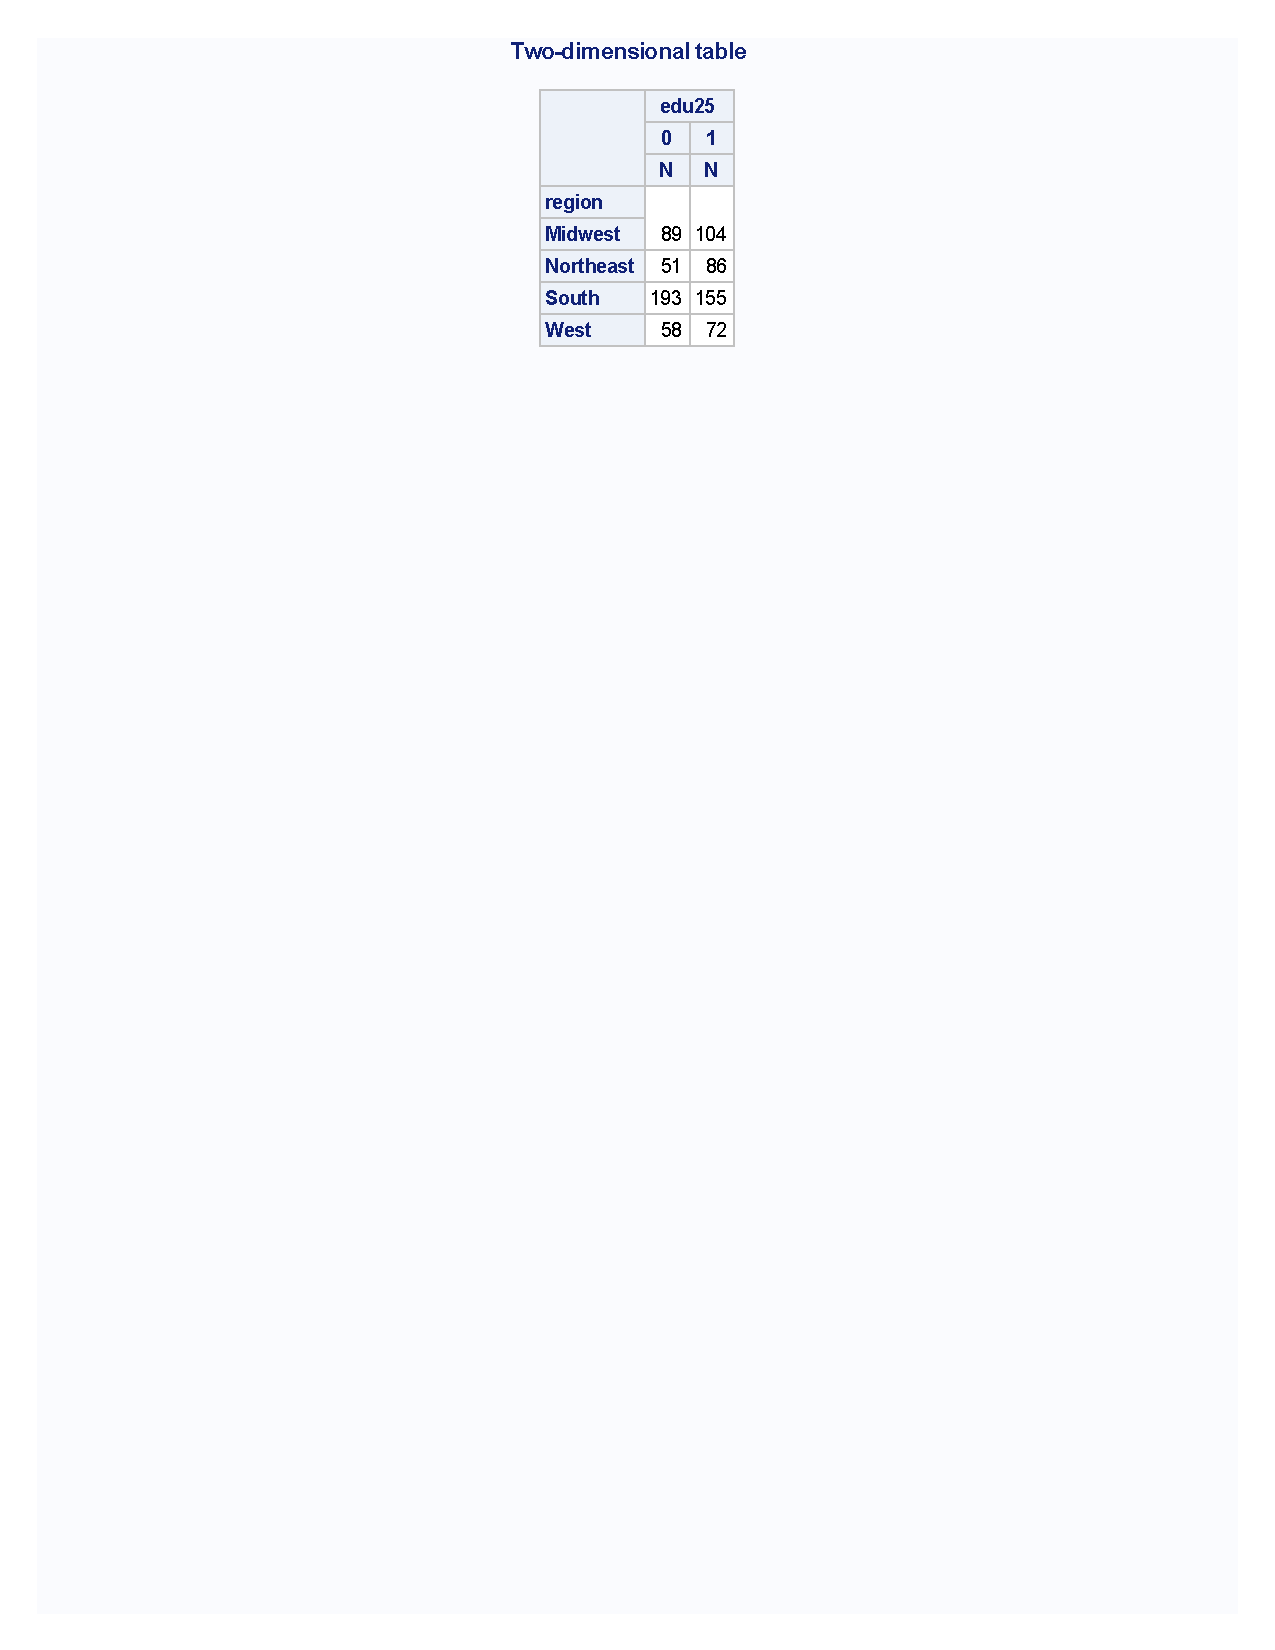
\includegraphics[trim={8.5cm 22cm 8.5cm 1.5cm},clip,width=1.0\textwidth]{L15_2dtable.pdf}
\emp
\blankcolumn
\bmp{0.6\textwidth}
\begin{clicker}{Which of the following is a correct interpretation?}
\begin{enumerate}
\item 72 people in the Western region with higher education levels received patents
\item 72 counties in the Western region with higher education levels received patents
\item 72 patents come from the Western region with higher education levels
\item 72\% of patents come the Western region with higher education levels
\end{enumerate}
\end{clicker}
\emp
\end{frame}


\begin{frame}[fragile]
\ft{Three-dimensional table}
\bmp{.60\textwidth}
\begin{code}{.}
PROC TABULATE DATA = patents ;
   CLASS unemp10 edu25 region ;
   TABLE unemp10, region, edu25 ;
RUN ;
\end{code}
\emp
\blankcolumn
\bmp{.40\textwidth}
\begin{itemize}
\item columns = \ttt{edu25}
\item rows = \ttt{region}
\item page = \ttt{unemp10}
\end{itemize}
\emp
\vspace{10pt}
\bmp{.50\textwidth}
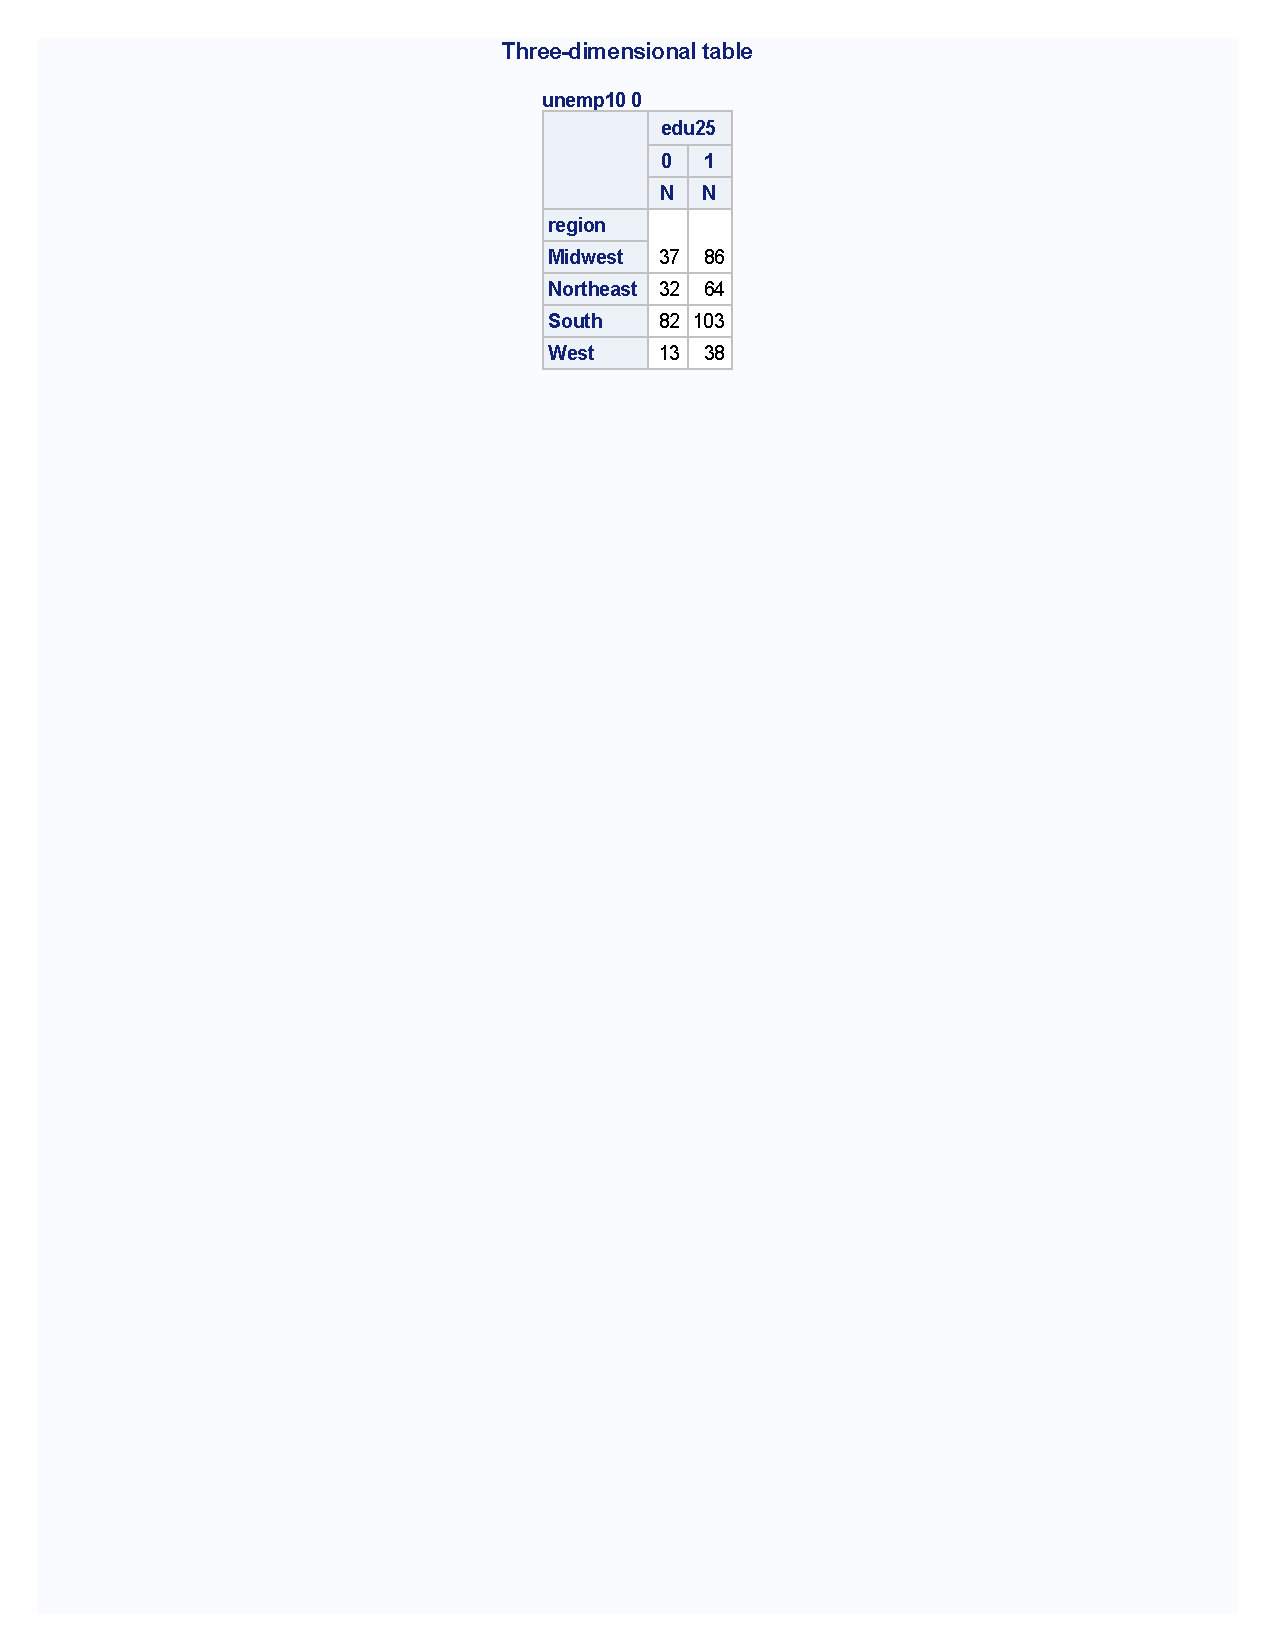
\includegraphics[trim={6.5cm 21cm 6.5cm 1.5cm},clip,width=1.0\textwidth]{L15_3dtable.pdf}
\emp
\blankcolumn
\bmp{.50\textwidth}
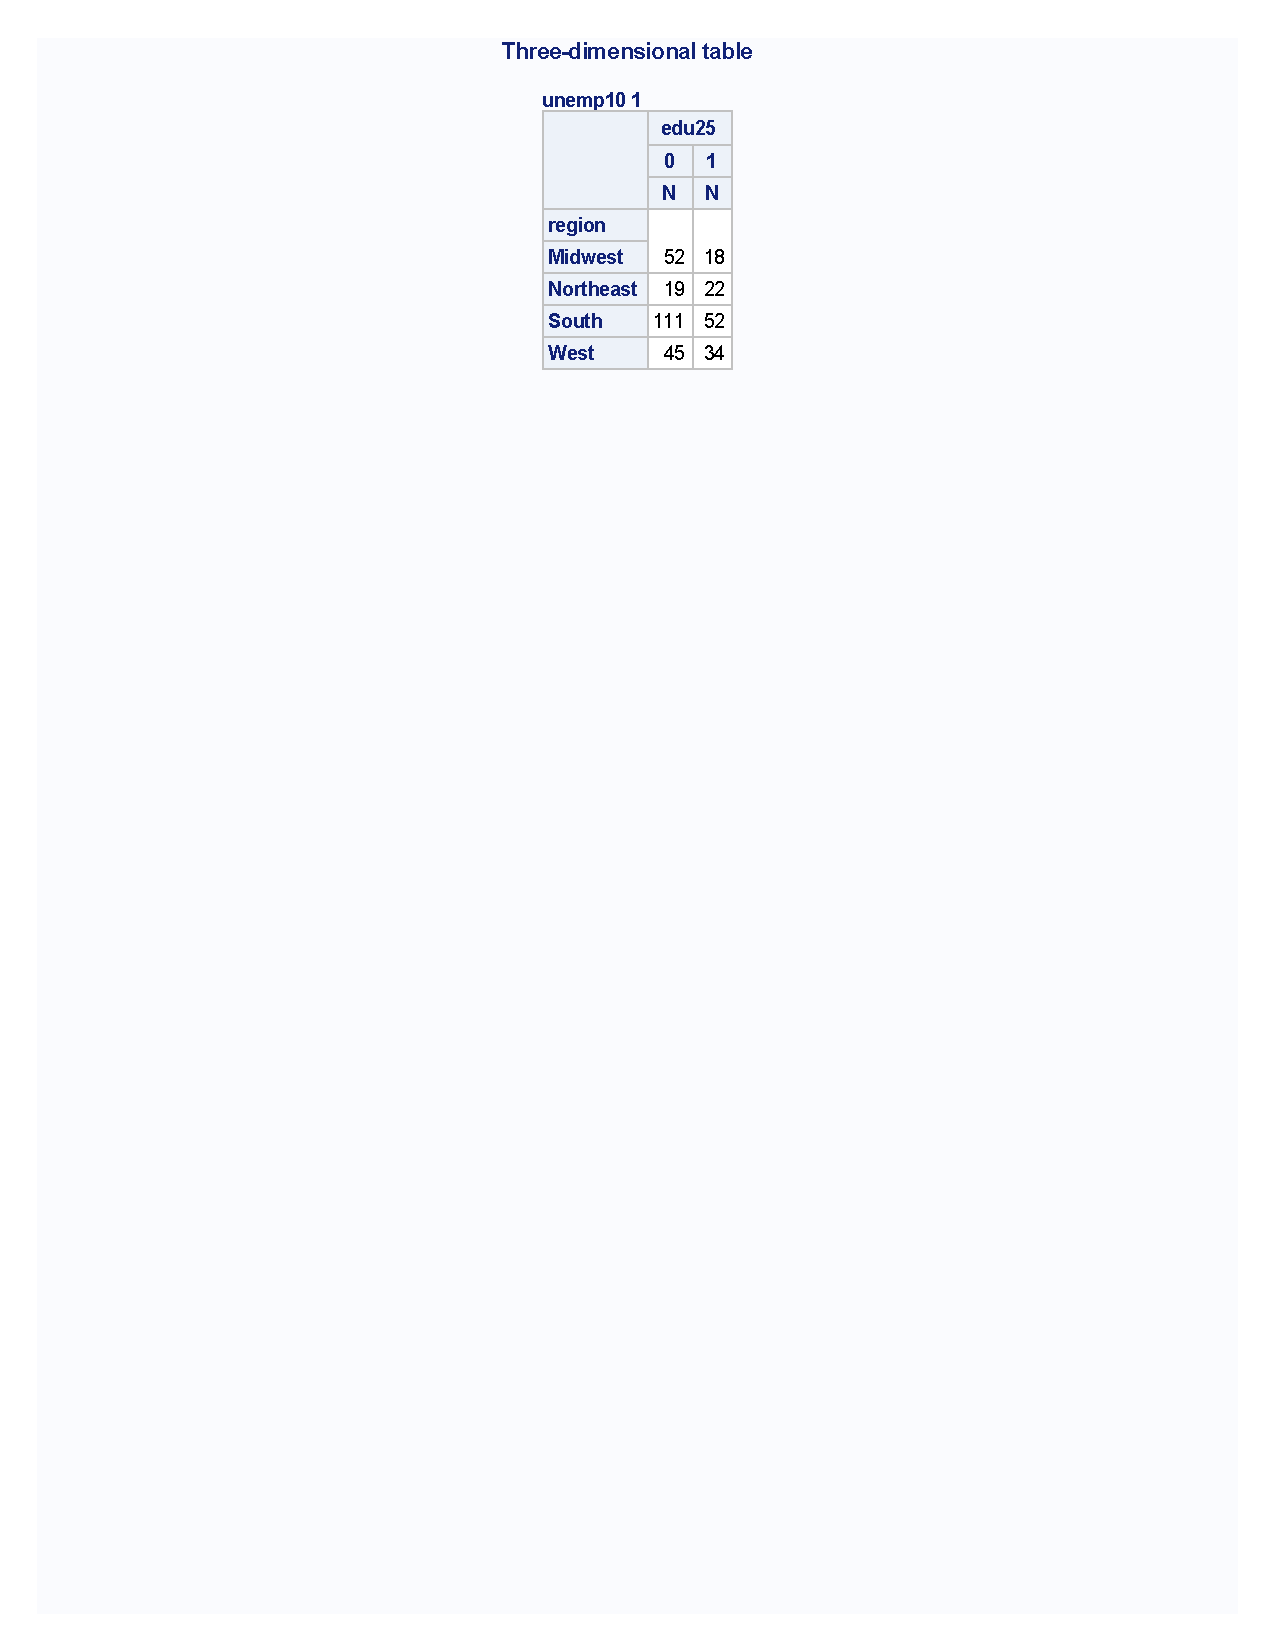
\includegraphics[trim={6.5cm 21cm 6.5cm 1.5cm},clip,width=1.0\textwidth]{L15_3dtable2.pdf}
\emp
\end{frame}



%\begin{frame}
%\ft{Concatenate vs Cross}
%\bi
%\item \emph{Concatenating} variables places them side by side
%\bi
%\item[] Syntax: separate variables by a space
%\item[] \fbox{\ttt{TABLE unemp10, \textcolor{OrangeRed}{edu25 region};}}
%\item[]
%\ei
%\item \emph{Crossing} variables nests values
%\bi
%\item[] Syntax: separate variables by an asterisk
%\item[] \fbox{\ttt{TABLE unemp10, \textcolor{OrangeRed}{edu25*region};}}
%\item[]
%\ei
%\item Don't forget!  Each variable listed in \ttt{TABLE} statement \ttb{must} also be listed in either \ttt{CLASS} or \ttt{VAR}.
%\ei
%\end{frame}

\begin{frame}[fragile]
\ft{Concatenate \hspace{1.5in} Cross}
\hspace*{-0.3in}
\bmp{.55\textwidth}
\begin{code}{.}
PROC TABULATE DATA = patents ;
   CLASS edu25 region unemp10 ;
   TABLE region, \textcolor{OrangeRed}{edu25 unemp10} ;
RUN ;
\end{code}
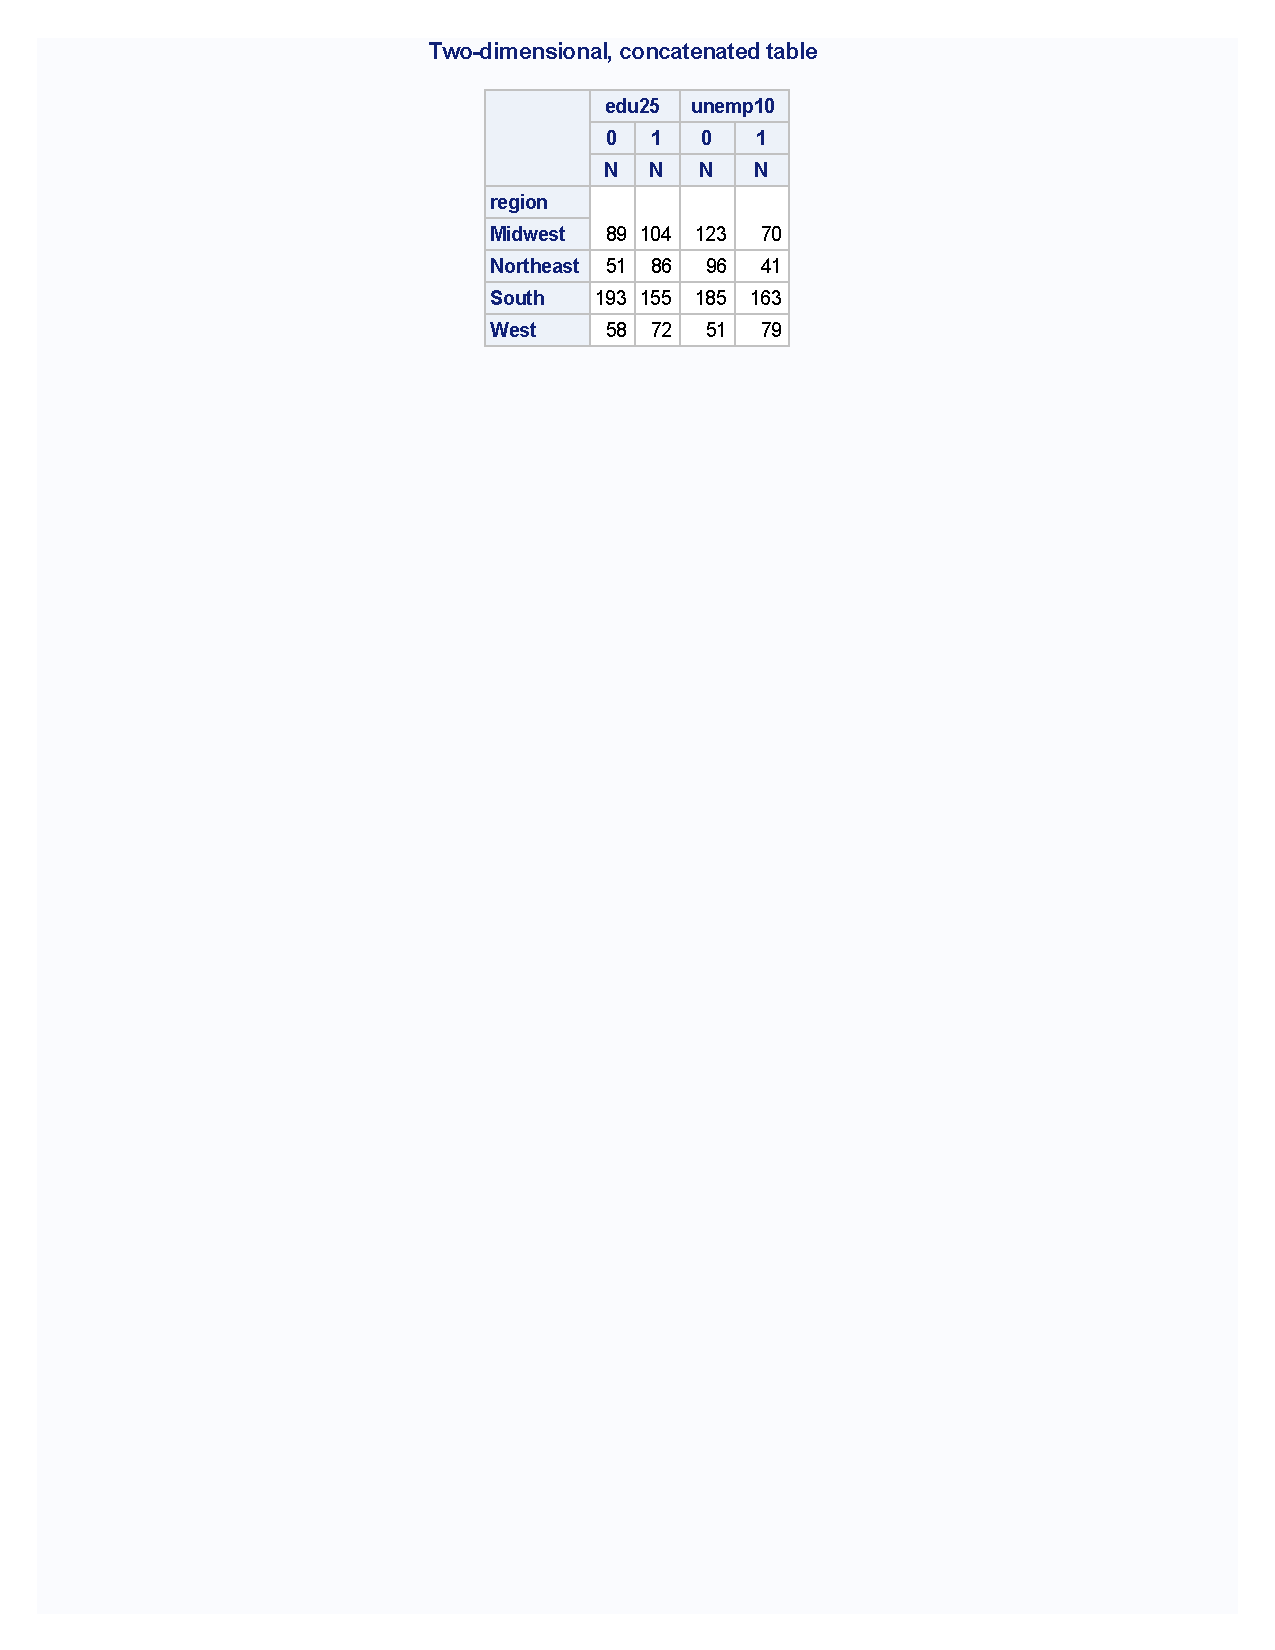
\includegraphics[trim={6.5cm 20cm 6.5cm 1.5cm},clip,width=1.0\textwidth]{L15_concatenate.pdf}
\emp
\blankcolumn
\bmp{.55\textwidth}
\begin{code}{.}
PROC TABULATE DATA = patents ;
   CLASS edu25 region unemp10 ;
   TABLE region, \textcolor{OrangeRed}{edu25*unemp10} ;
RUN ;
\end{code}
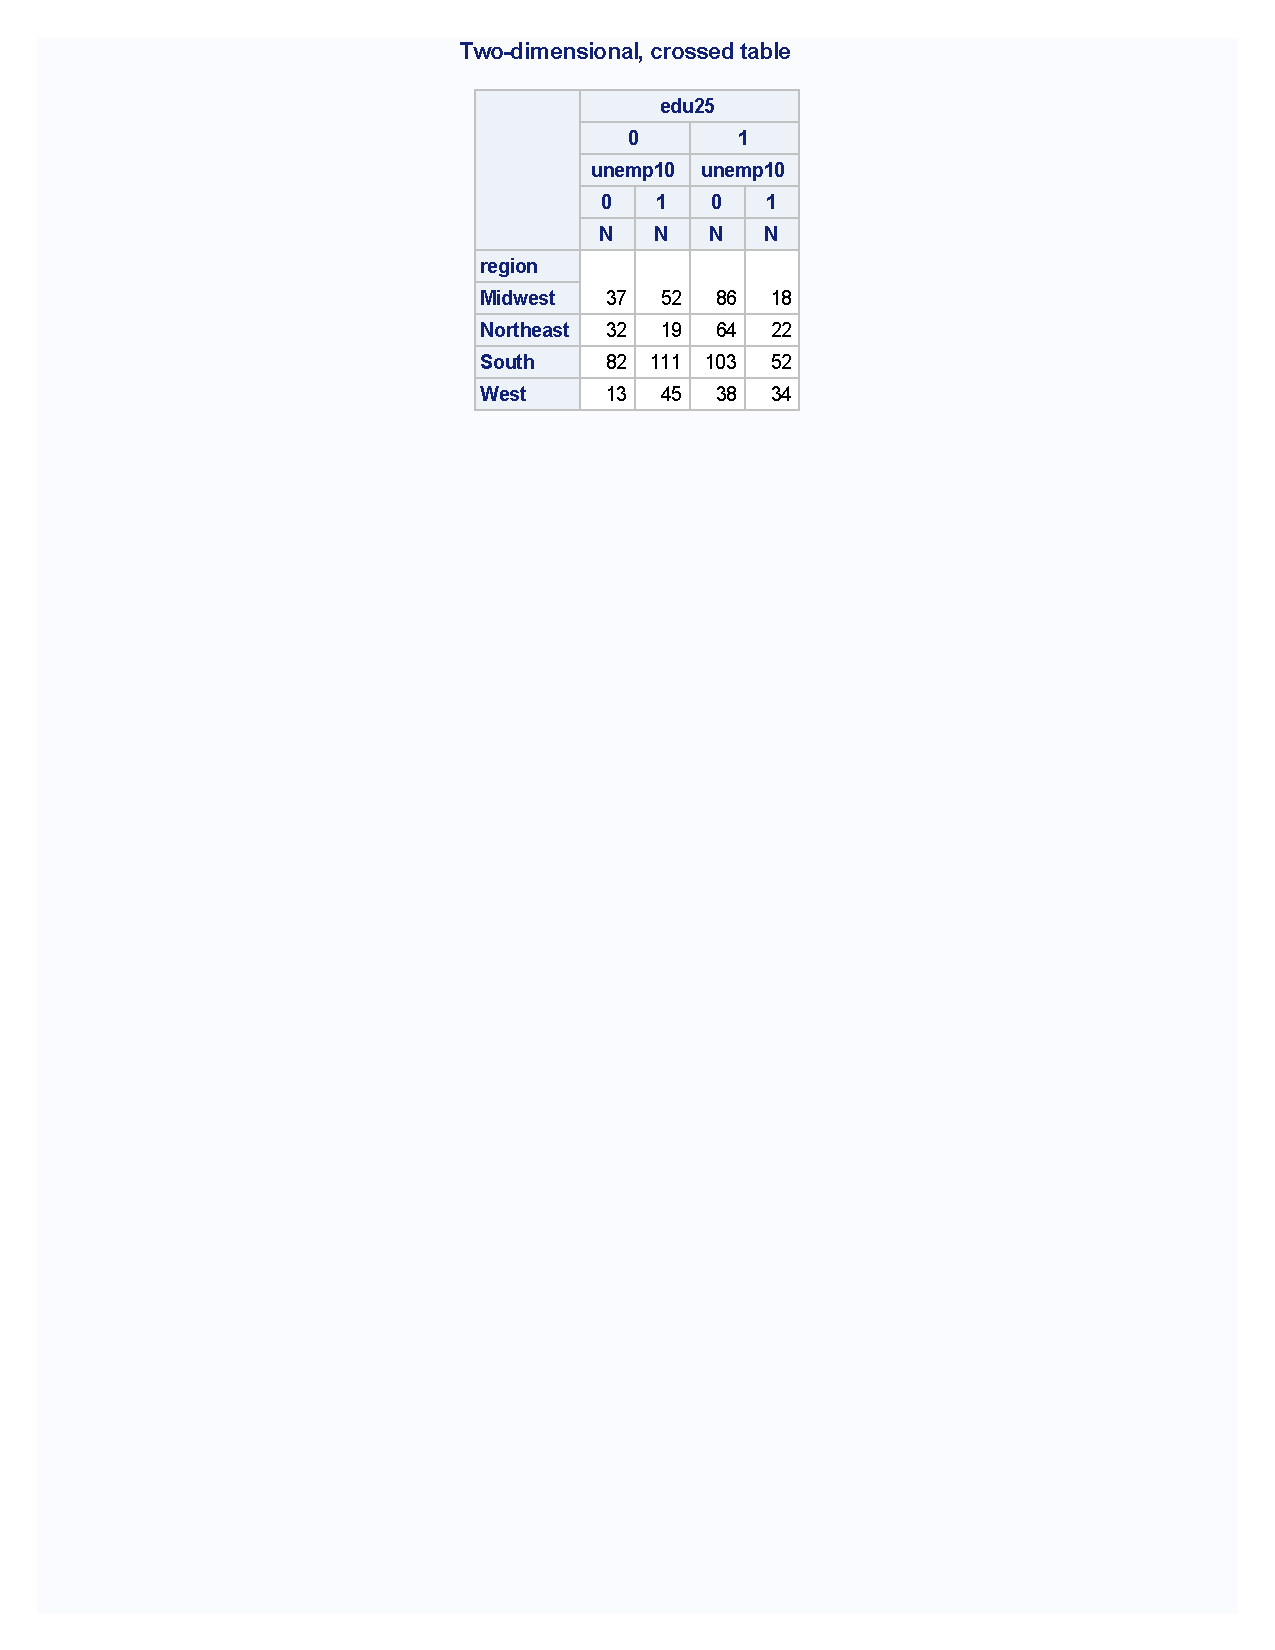
\includegraphics[trim={6.5cm 20cm 6.5cm 1.5cm},clip,width=1.0\textwidth]{L15_cross.pdf}
\emp
\end{frame}



\begin{frame}
\ft{Discussion}
\bmp{0.38\textwidth}
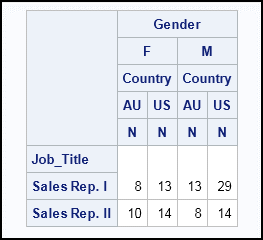
\includegraphics[trim={0.2cm 0.2cm 0.2cm 0.2cm},clip,width=1.0\textwidth]{table1.png}
\emp
\bmp{0.05\textwidth} \hspace{0.05in} \emp
\bmp{0.60\textwidth}
\oyo This is a \underline{(one/two/three)} dimensional table where the variables \ttt{gender} and \ttt{country} are \underline{(crossed/concatenated)}.
\emp
\begin{clicker}{The statement that generated this table is:}
\begin{enumerate}
\item \ttt{TABLE country*gender, job\_title ;}
\item \ttt{TABLE job\_title, gender*country ;}
\item \ttt{TABLE gender, country, job\_title ;}
\item \ttt{TABLE job\_title, country gender ;}
\item \ttt{TABLE country gender, job\_title ;}
\end{enumerate}
\end{clicker}
\end{frame}

\begin{frame}
\ft{Creating totals}
The keyword \ttt{ALL} can be used to create \emph{overall} summarizations.
\vskip5pt
\bi
\item \ttt{ALL} can be included in any table dimension
\item[] \fbox{\ttt{TABLE region ALL, edu25 ALL;}}
\item[]
\item \ttt{ALL} can be included with concatenated variables
\item[] \fbox{\ttt{TABLE region, edu25 ALL unemp10 ALL;}}
\item[]
\item \ttt{ALL} can be included with crossed variables
\item[] \fbox{\ttt{TABLE region, edu25*unemp10 ALL;}}
\item[]
\item use parentheses to summarize within group(s)
\item[] \fbox{\ttt{TABLE region, edu25*(unemp10 ALL) ALL;}}
\ei
\end{frame}

\begin{frame}[fragile]
\ft{Example with ALL}
\bmp{.75\textwidth}
\begin{code}{.}
PROC TABULATE DATA = patents;
   CLASS edu25 region unemp10;
   TABLE region, edu25*(unemp10 \textcolor{OrangeRed}{ALL}) \textcolor{OrangeRed}{ALL} ;
RUN;
\end{code}
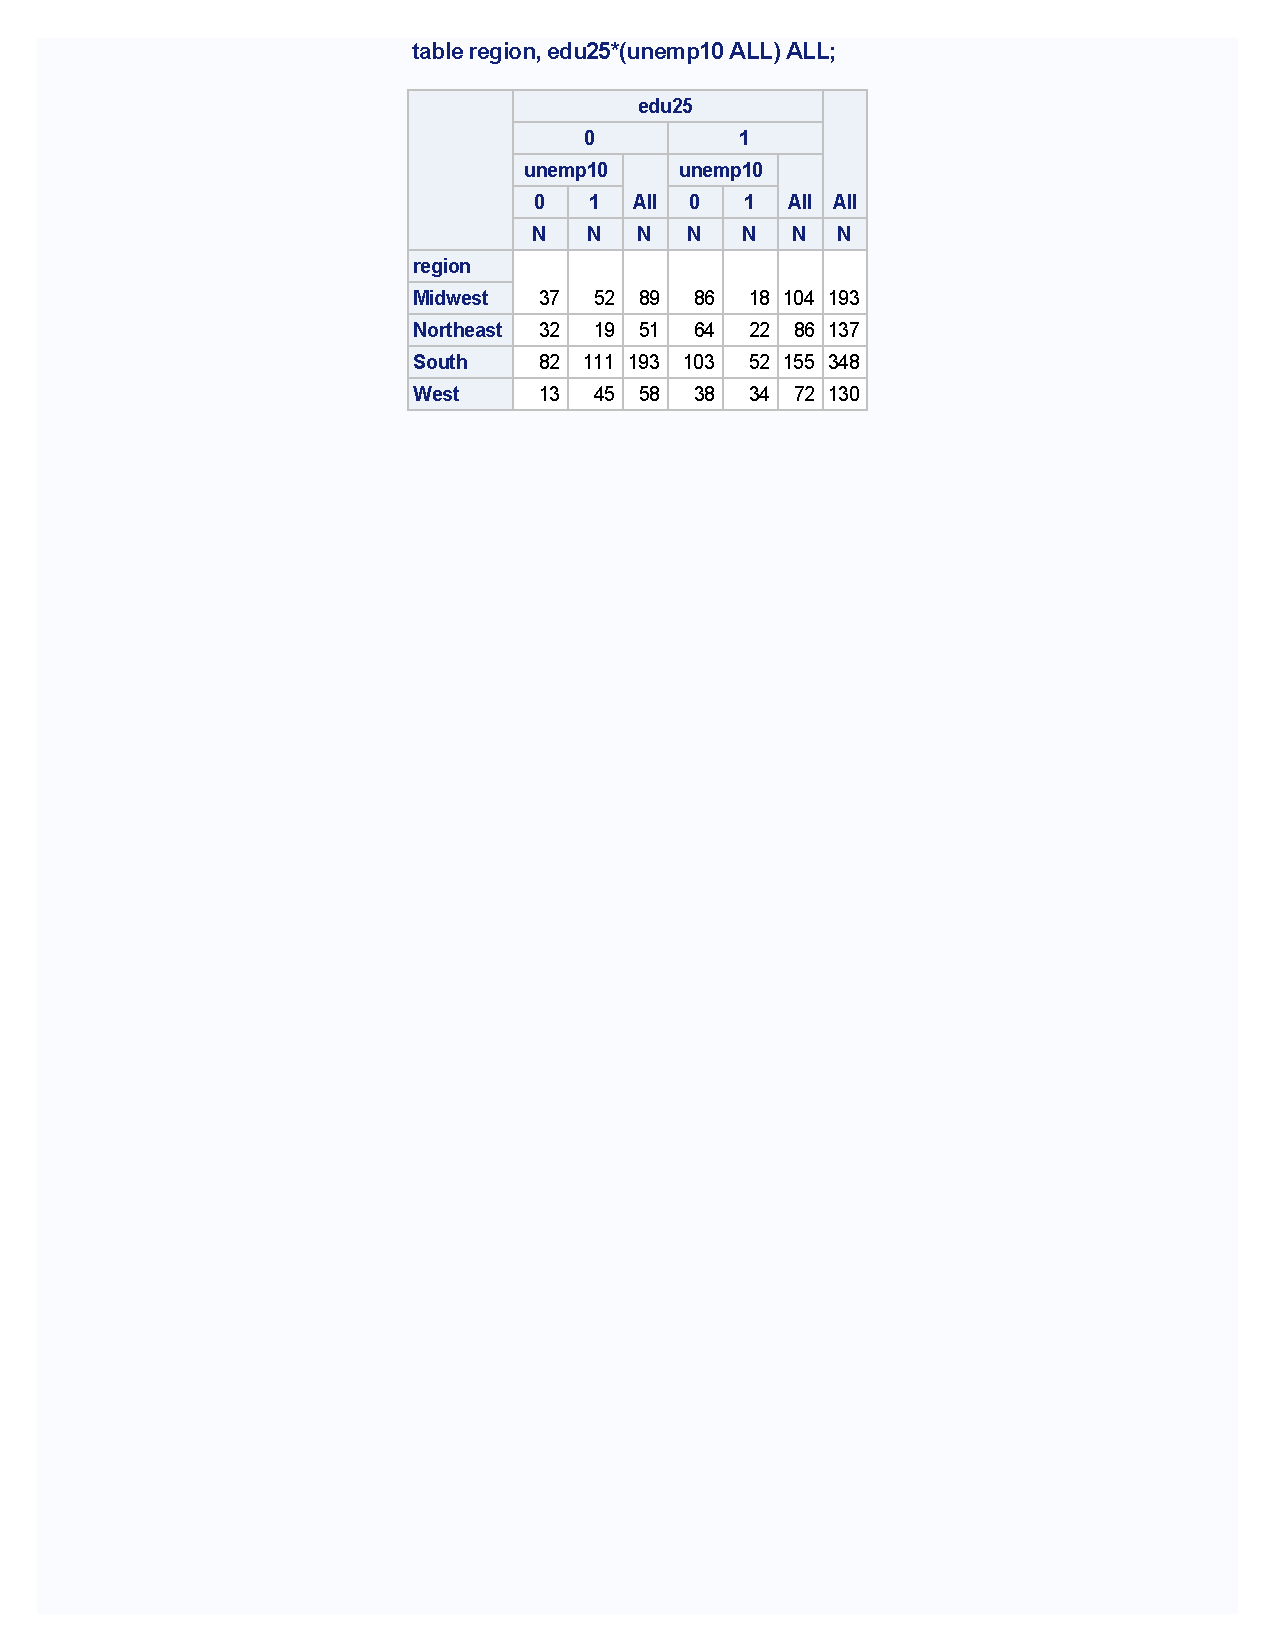
\includegraphics[trim={5cm 20cm 5cm 1.5cm},clip,width=1.0\textwidth]{L15_ALLexample.pdf}
\emp
\end{frame}



%===========================================================================================================================
\section[Statistics]{Statistics}
%===========================================================================================================================
\subsection{}
\begin{frame}
\tableofcontents[currentsection, hideallsubsections]
\end{frame}


\begin{frame}[fragile]
\ft{Categorical variables - default statistics}
\hspace*{-0.3in}
\bmp{0.52\textwidth}
\begin{code}{.}
PROC TABULATE DATA = patents ;
   CLASS \textcolor{OrangeRed}{edu25} region ;
   TABLE region, \textcolor{OrangeRed}{edu25} ;
RUN ;
\end{code}
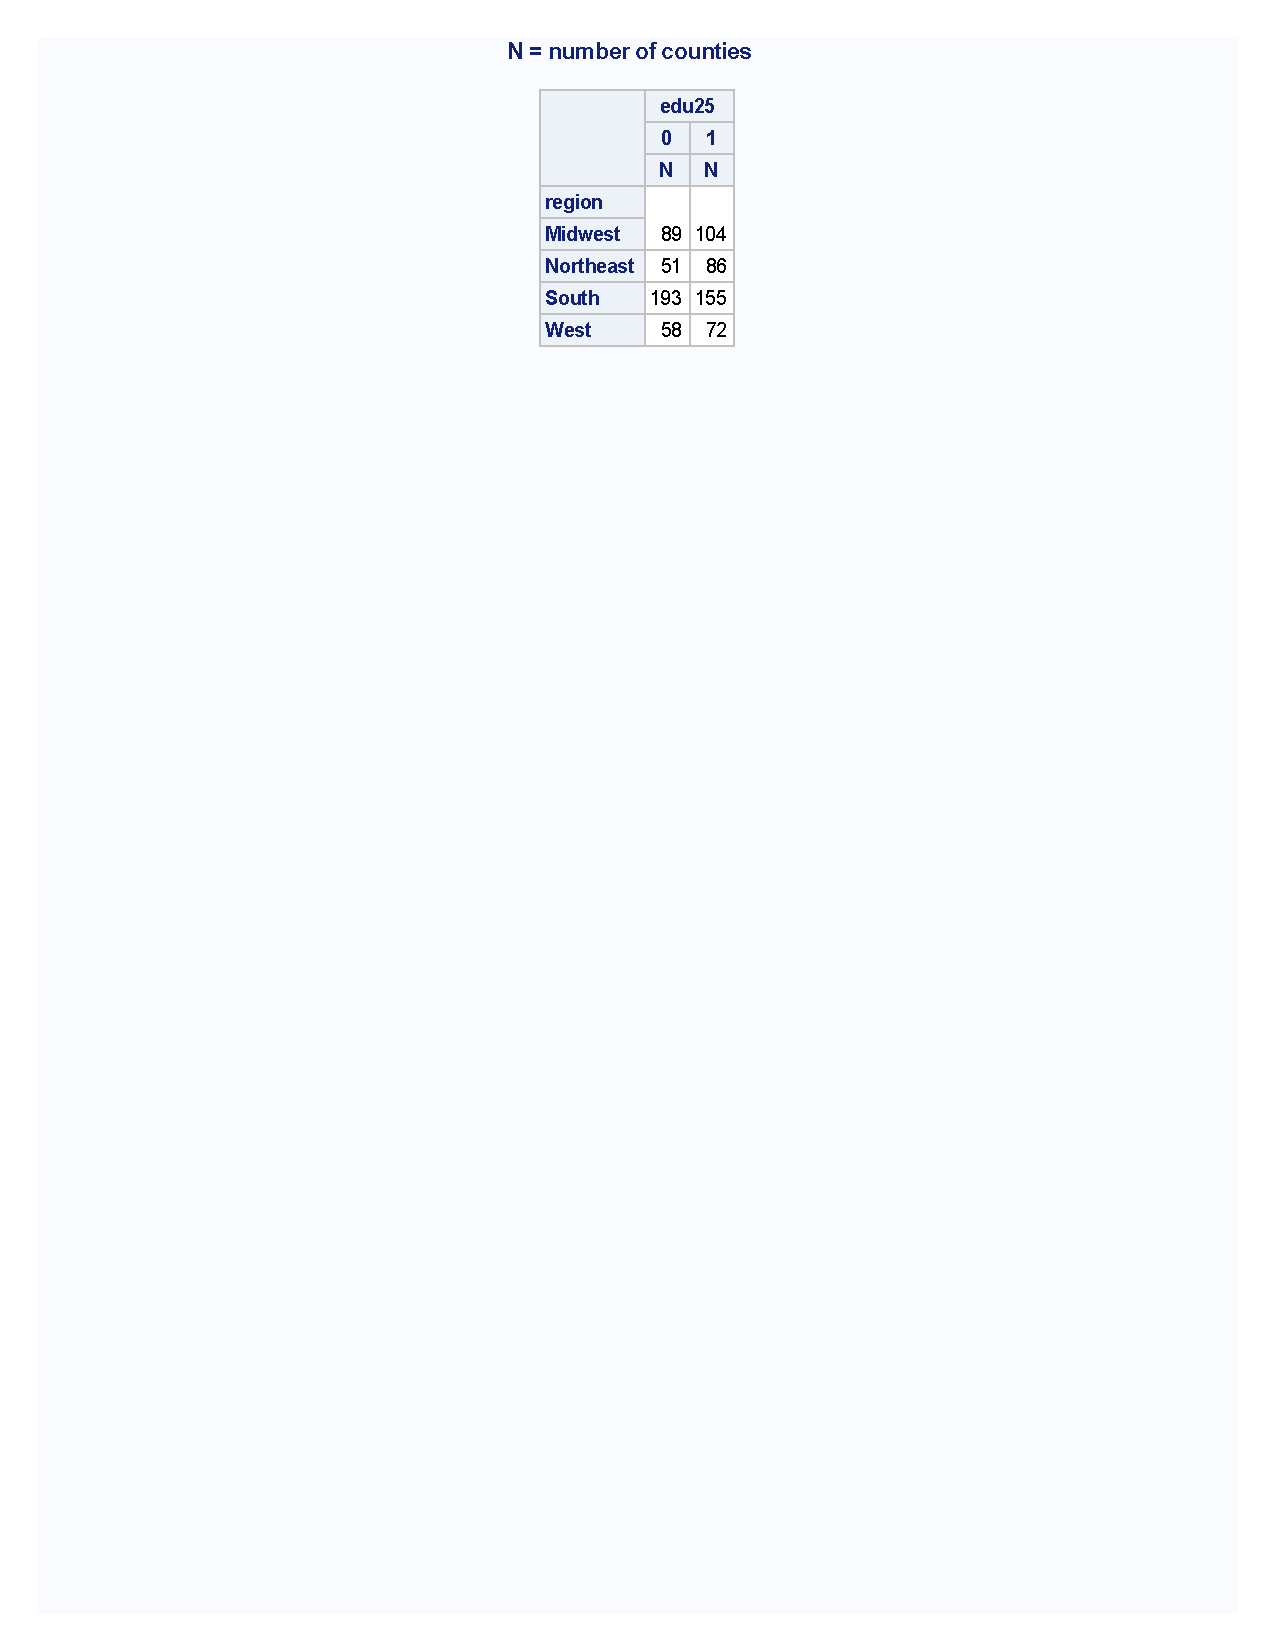
\includegraphics[trim={7cm 21cm 7cm 1.5cm},clip,width=1.0\textwidth]{L15_catstats.pdf}
\emp
\blankcolumn
\bmp{0.52\textwidth}
\begin{code}{.}
PROC TABULATE DATA = patents ;
   CLASS \textcolor{OrangeRed}{edu25} region ;
   TABLE region, \textcolor{OrangeRed}{edu25*N} ;
RUN ;
\end{code}
\bi
\item categorical variables go in \ttt{CLASS}
\item default statistic is $N$
\item $N$ can be explicitly specified with \ttt{*}
\item[]
\item[]
\ei
\emp
\end{frame}


\begin{frame}[fragile]
\ft{Quantitative variables - default statistics}
\hspace*{-0.3in}
\bmp{0.52\textwidth}
\begin{code}{.}
PROC TABULATE DATA = patents ;
   CLASS region ;
   VAR \textcolor{OrangeRed}{patents} ;
   TABLE region, \textcolor{OrangeRed}{patents} ;
RUN;
\end{code}
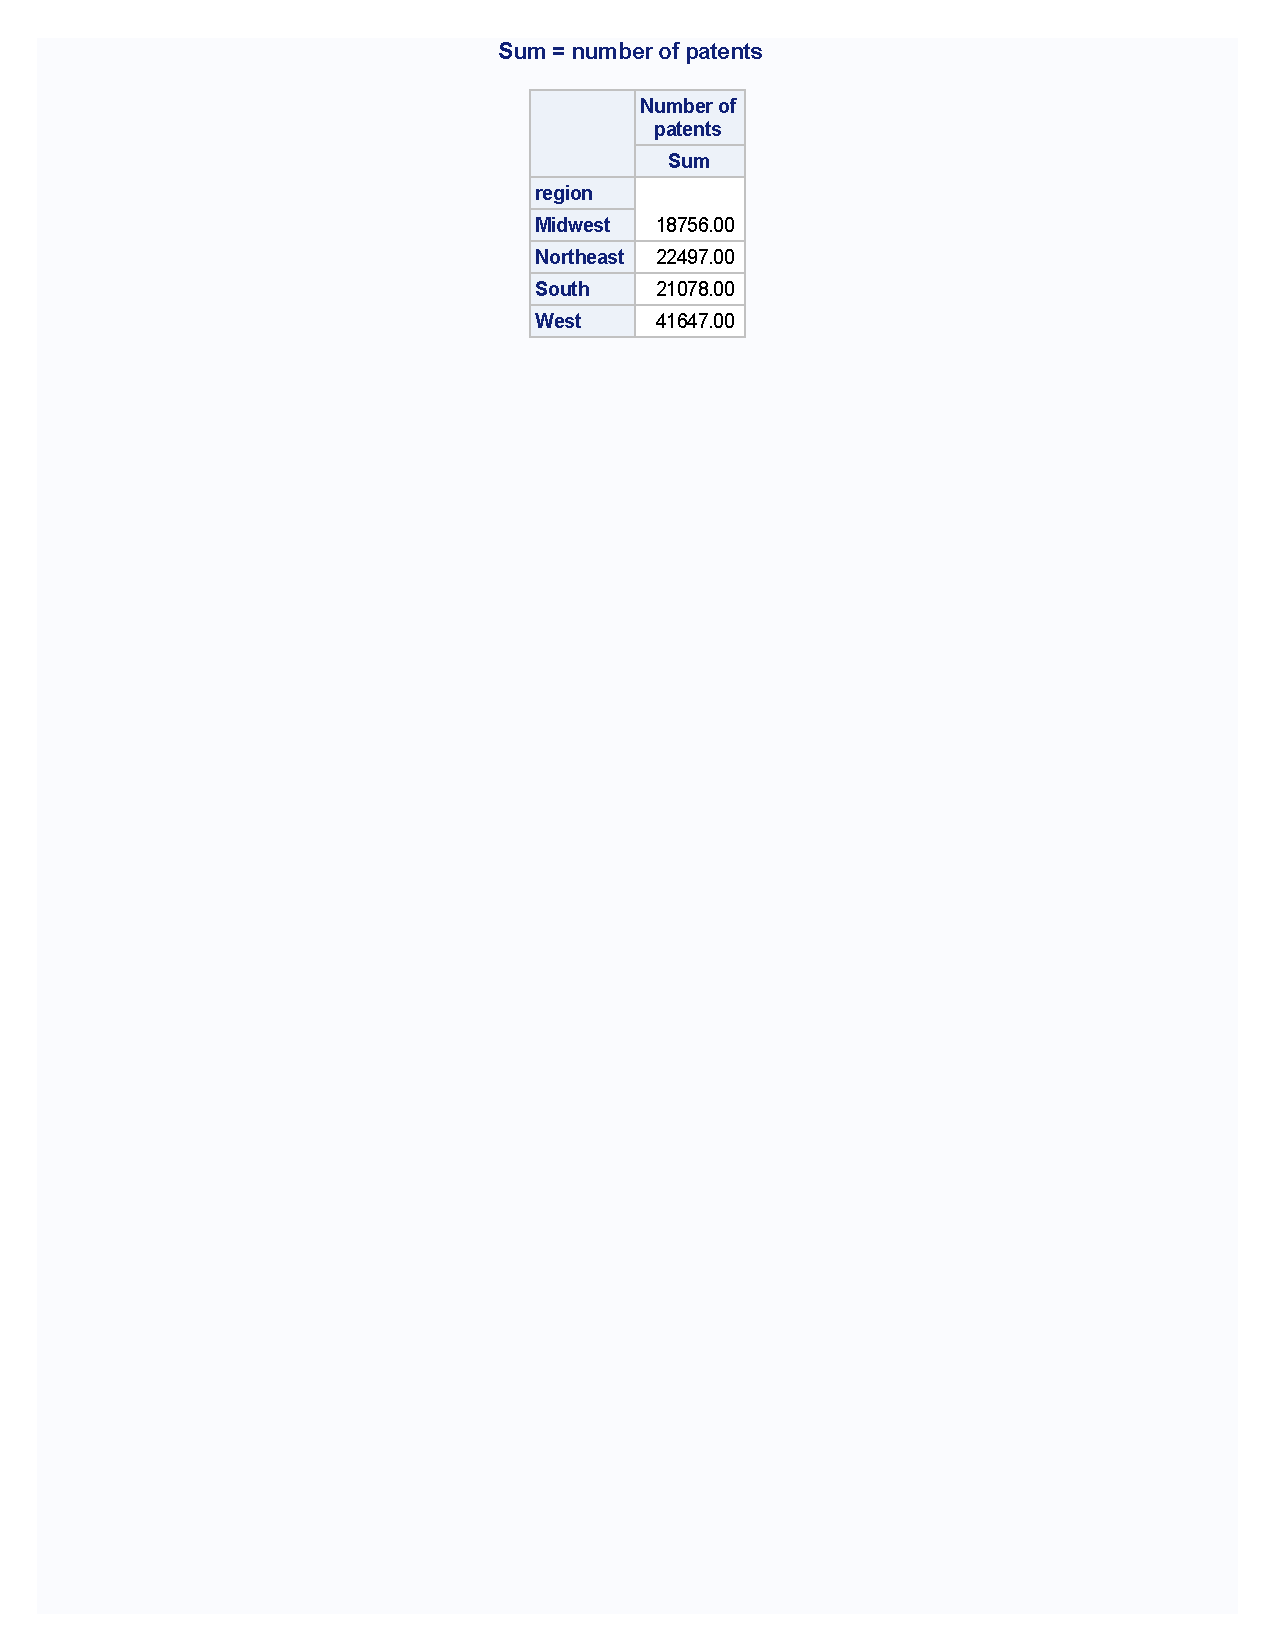
\includegraphics[trim={7cm 21cm 7cm 1.5cm},clip,width=1.0\textwidth]{L15_quantstats.pdf}
\emp
\blankcolumn
\bmp{0.52\textwidth}
\begin{code}{.}
PROC TABULATE DATA = patents ;
   CLASS region ;
   VAR \textcolor{OrangeRed}{patents} ;
   TABLE region, \textcolor{OrangeRed}{patents*SUM} ;
RUN ;
\end{code}
\bi
\item quantitative variables go in \ttt{VAR}
\item default statistic is $SUM$
\item $SUM$ can be explicitly specified with \ttt{*}
\item[]
\item[]
\ei
\emp
\end{frame}




\begin{frame}[fragile]
\ft{Specifying Statistics}
\hspace*{-0.2in}
\bmp{0.65\textwidth}
\begin{code}{.}
PROC TABULATE data = patents ;
   CLASS edu25 region ;
   VAR patents ;
   TABLE region,
         edu25*patents*(N SUM MEAN) ;
RUN ;
\end{code}
\emp
\blankcolumn
\bmp{0.40\textwidth}
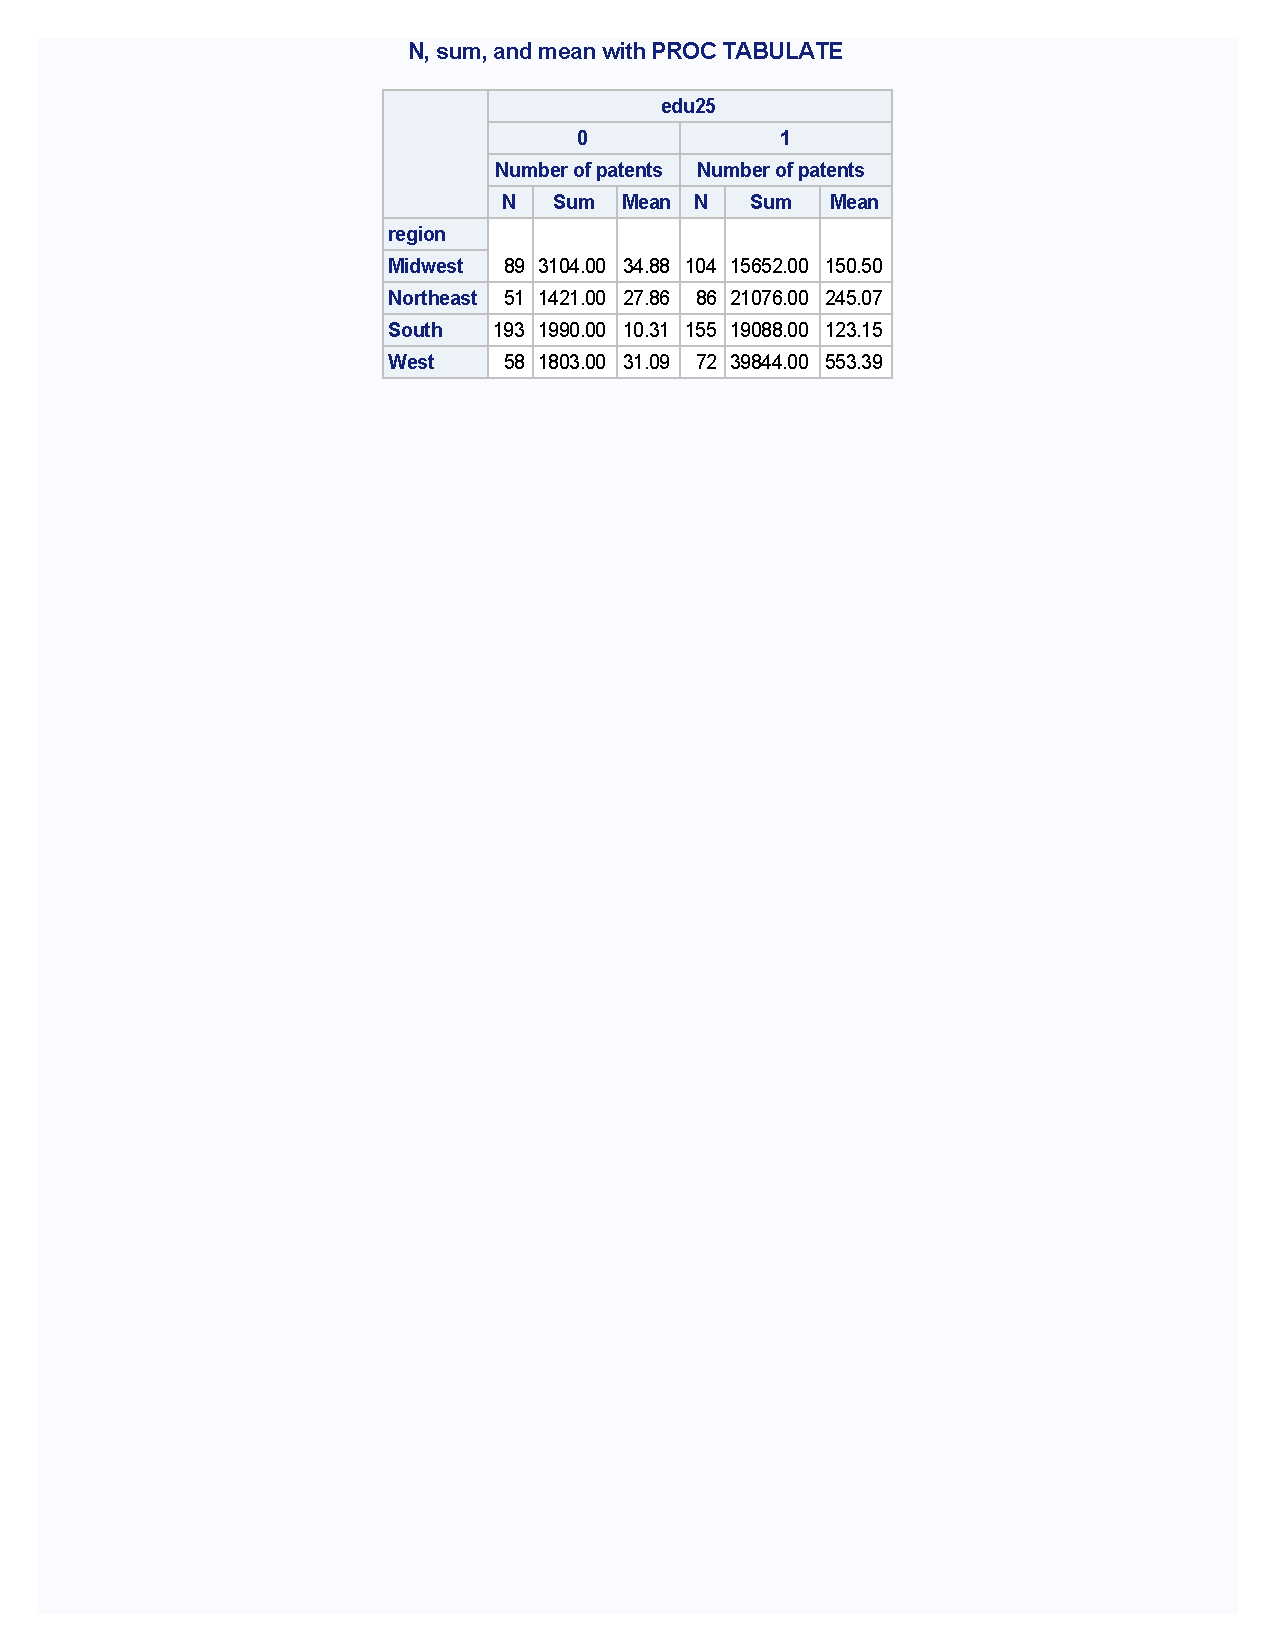
\includegraphics[trim={6cm 21cm 6cm 1.5cm},clip,width=1.0\textwidth]{L15_nestedstats.pdf}
\emp
\bi
\item[]
\item A statistic is specified in \ttt{TABLE} dimension with \ttt{*}
\item[] \fbox{\ttt{TABLE \emph{quantvar}*\textcolor{OrangeRed}{\emph{statistic}};}}
\item Nest statistic within \emph{catvar}
\item[] \fbox{\ttt{TABLE \emph{catvar}*\emph{quantvar}*\textcolor{OrangeRed}{\emph{statistic}};}}
\item Multiple statistics can be specified with parentheses
\item[] \fbox{\ttt{TABLE region, edu25*patents*(\textcolor{OrangeRed}{N SUM MEAN});}}
\ei
\end{frame}

\begin{frame}
\ft{TABLE statistics}
\begin{center}
\resizebox{1.0\textwidth}{!}{
\begin{tabular}{lllll}
CSS & CV & KURTOSIS & LCLM & MAX \\
MEAN & MIN & MODE & N & NMISS \\
RANGE & SKEWNESS & STDEV & STDERR & SUM \\
SUMWGT & UCLM & USS & VAR \\
PCTN & PCTSUM & REPPCTN & REPPCTSUM & PAGEPCTN \\
PAGEPCTSUM & ROWPCTN & ROWPCTSUM & COLPCTN & COLPCTSUM \\
MEDIAN & P1 & P5 & P10 & P25  \\
P75 & P90 & P95 & P99 & QRANGE  \\
\end{tabular}}
\end{center}
\end{frame}



\begin{frame}[fragile]
\ft{Statistics with ALL}
\bmp{0.75\textwidth}
\begin{code}{.}
PROC TABULATE DATA = patents ;
  CLASS edu25 region ;
  VAR patents ;
  TABLE region \textcolor{OrangeRed}{ALL},
        edu25*patents*(N SUM MEAN ROWPCTSUM)
        \textcolor{OrangeRed}{ALL}*patents*(N SUM MEAN ROWPCTSUM) ;
RUN ;
\end{code}
\emp
\vspace{10pt}
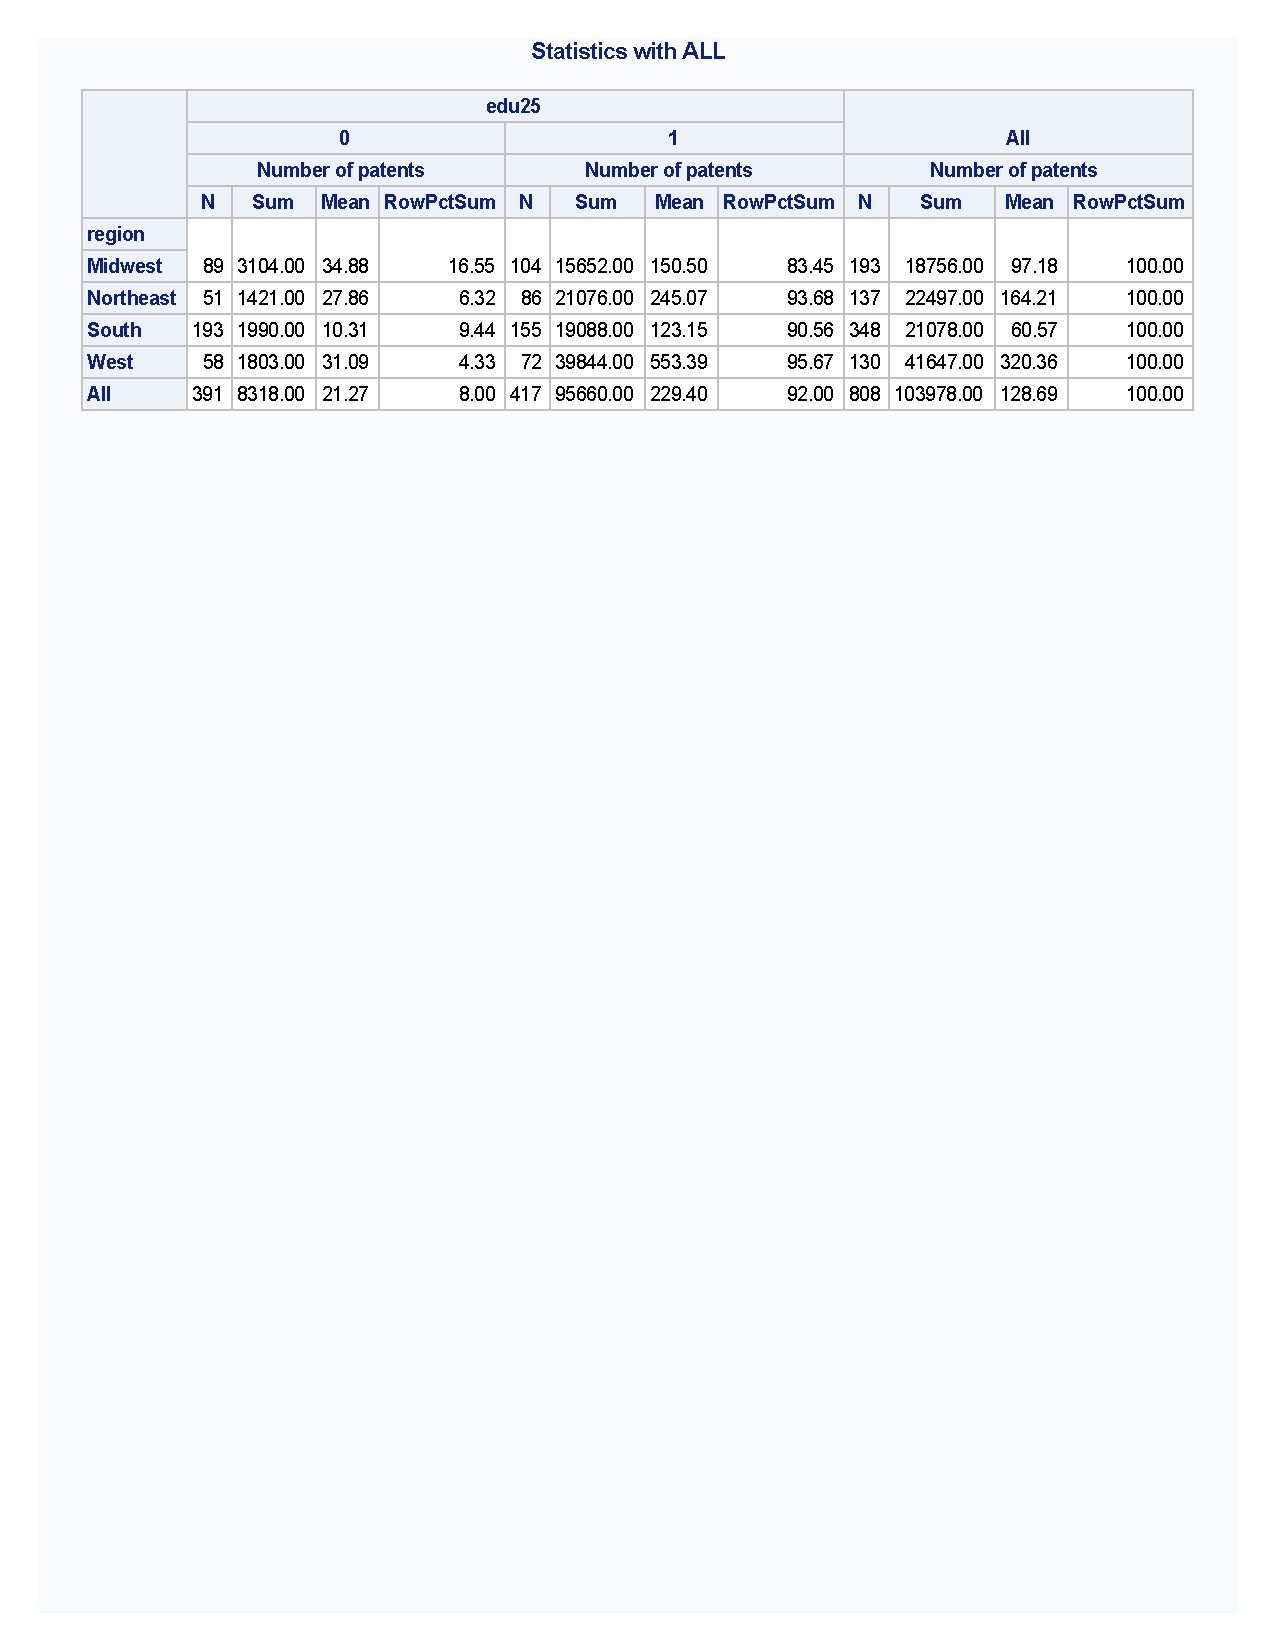
\includegraphics[trim={1cm 20cm 1cm 1.5cm},clip,width=0.8\textwidth]{L15_ALLstats.pdf}

%\blankcolumn
%\bmp{0.25\textwidth}
%\bi
%\item  \ttt{ALL} - returns $N$
%\item  \ttt{ALL*\emph{quantvar}} - returns $SUM$
%\item \ttt{ALL*\emph{quantvar}*\emph{statistic}} - returns \emph{statistic}
%\ei
%\emp


\end{frame}


\begin{frame}
\ft{Discussion}
\bmp{0.43\textwidth}
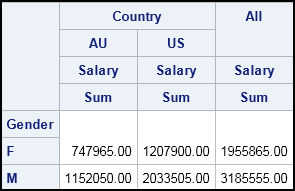
\includegraphics[trim={0.1cm 0.1cm 0.1cm 0.1cm},clip,width=0.80\textwidth]{table2.png}
\emp
\\
\begin{clicker}{The statement that generated this table is:}
\begin{enumerate}
\item \ttt{TABLE gender, country, ALL ;}
\item \ttt{TABLE gender, country, ALL*salary ;}
\item \ttt{TABLE gender, country*salary ALL ;}
\item \ttt{TABLE gender, country*salary ALL*salary ;}
\item \ttt{TABLE gender, country*SUM, ALL*SUM ;}
\end{enumerate}
\end{clicker}
\end{frame}


%===========================================================================================================================
\section[Display]{Display}
%===========================================================================================================================
\subsection{}
\begin{frame}
\tableofcontents[currentsection, hideallsubsections]
\end{frame}

\begin{frame}
\ft{Discussion}
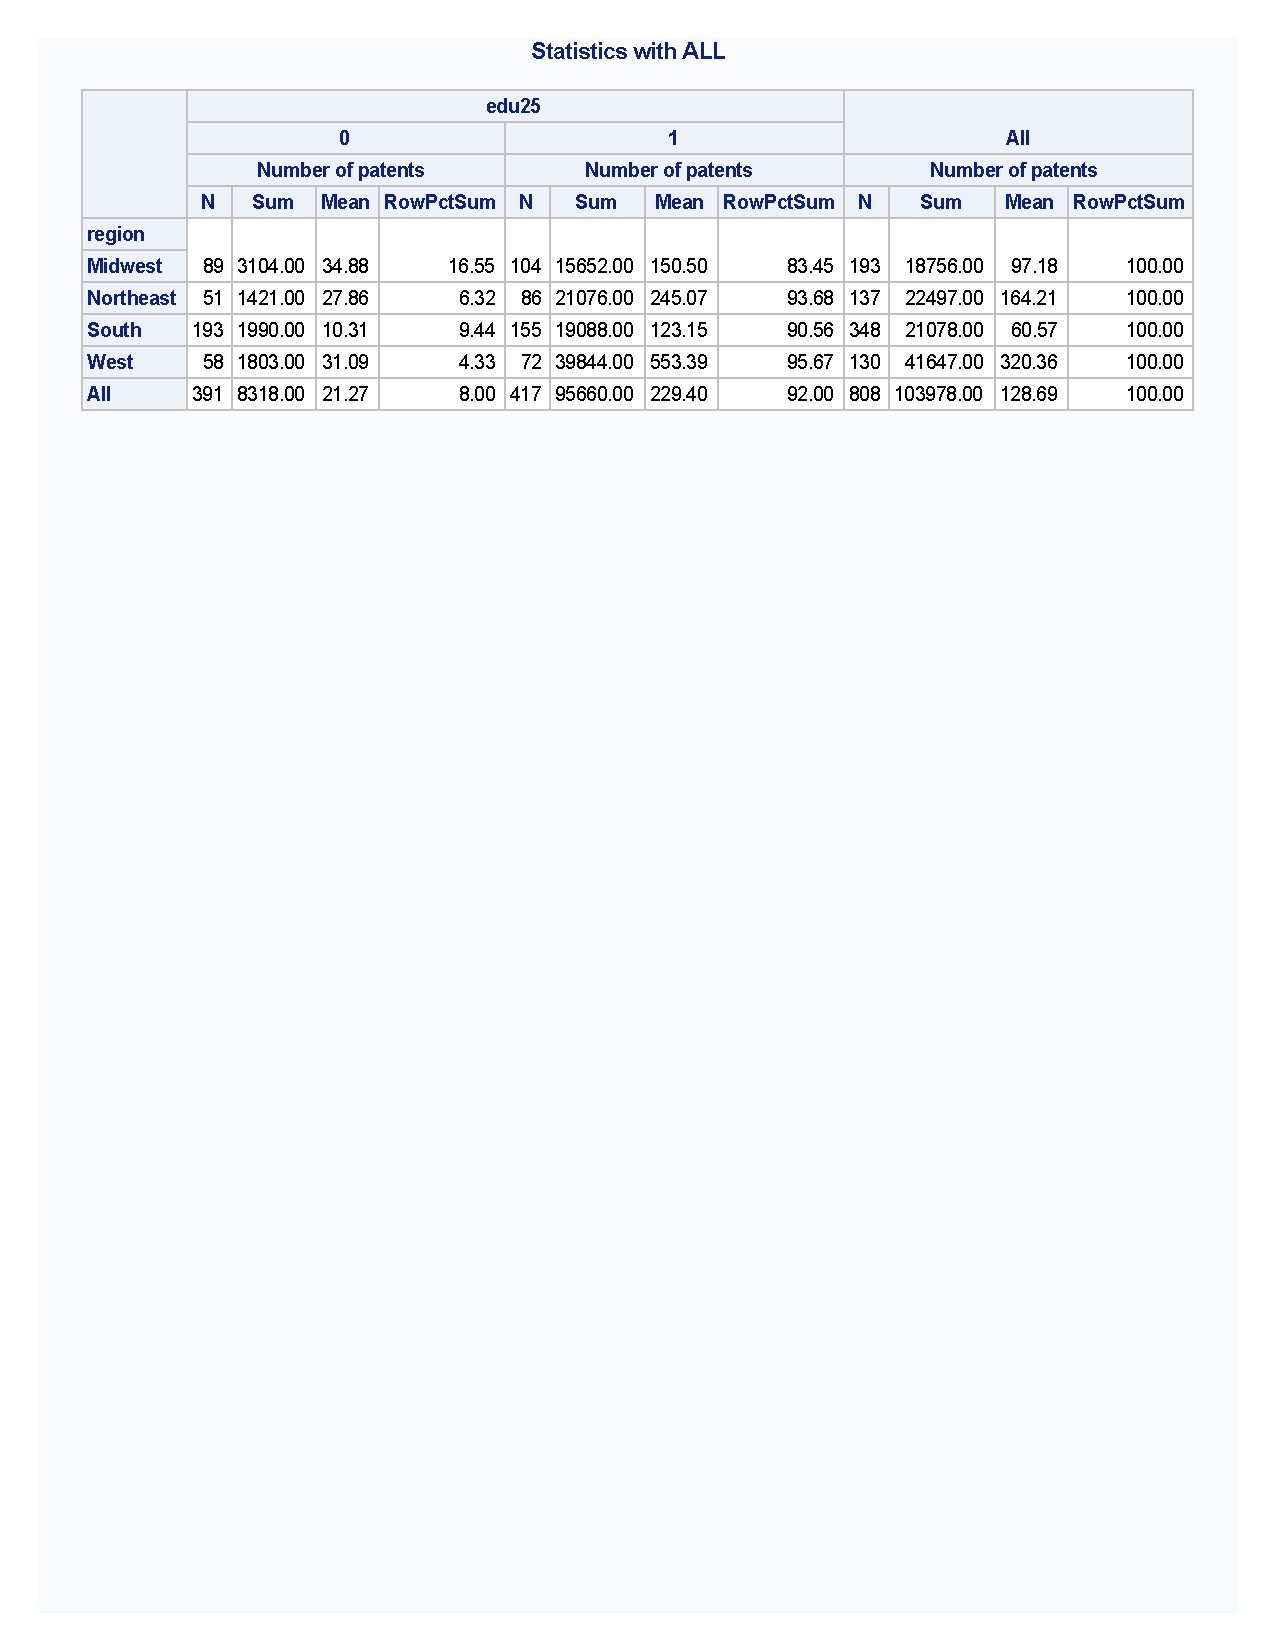
\includegraphics[trim={1cm 20cm 1cm 1.5cm},clip,width=1.0\textwidth]{L15_ALLstats.pdf}\\
\vskip10pt
\oyo What are some things you would like to change about this table?
\end{frame}

\begin{frame}[fragile]
\ft{Apply formats to variable values}
\bmp{1.0\textwidth}
\begin{code}{.}
PROC FORMAT ;  VALUE yn 1 = "Yes" 0 = "No" ; RUN ;
PROC TABULATE DATA = patents ;
   CLASS edu25 region;
   VAR patents;
   TABLE region ALL,
         edu25*patents*(N SUM MEAN ROWPCTSUM)
         ALL*patents*(N SUM MEAN ROWPCTSUM);
    \textcolor{OrangeRed}{FORMAT edu25 yn. ;}
RUN;
\end{code}
\emp
\vskip10pt
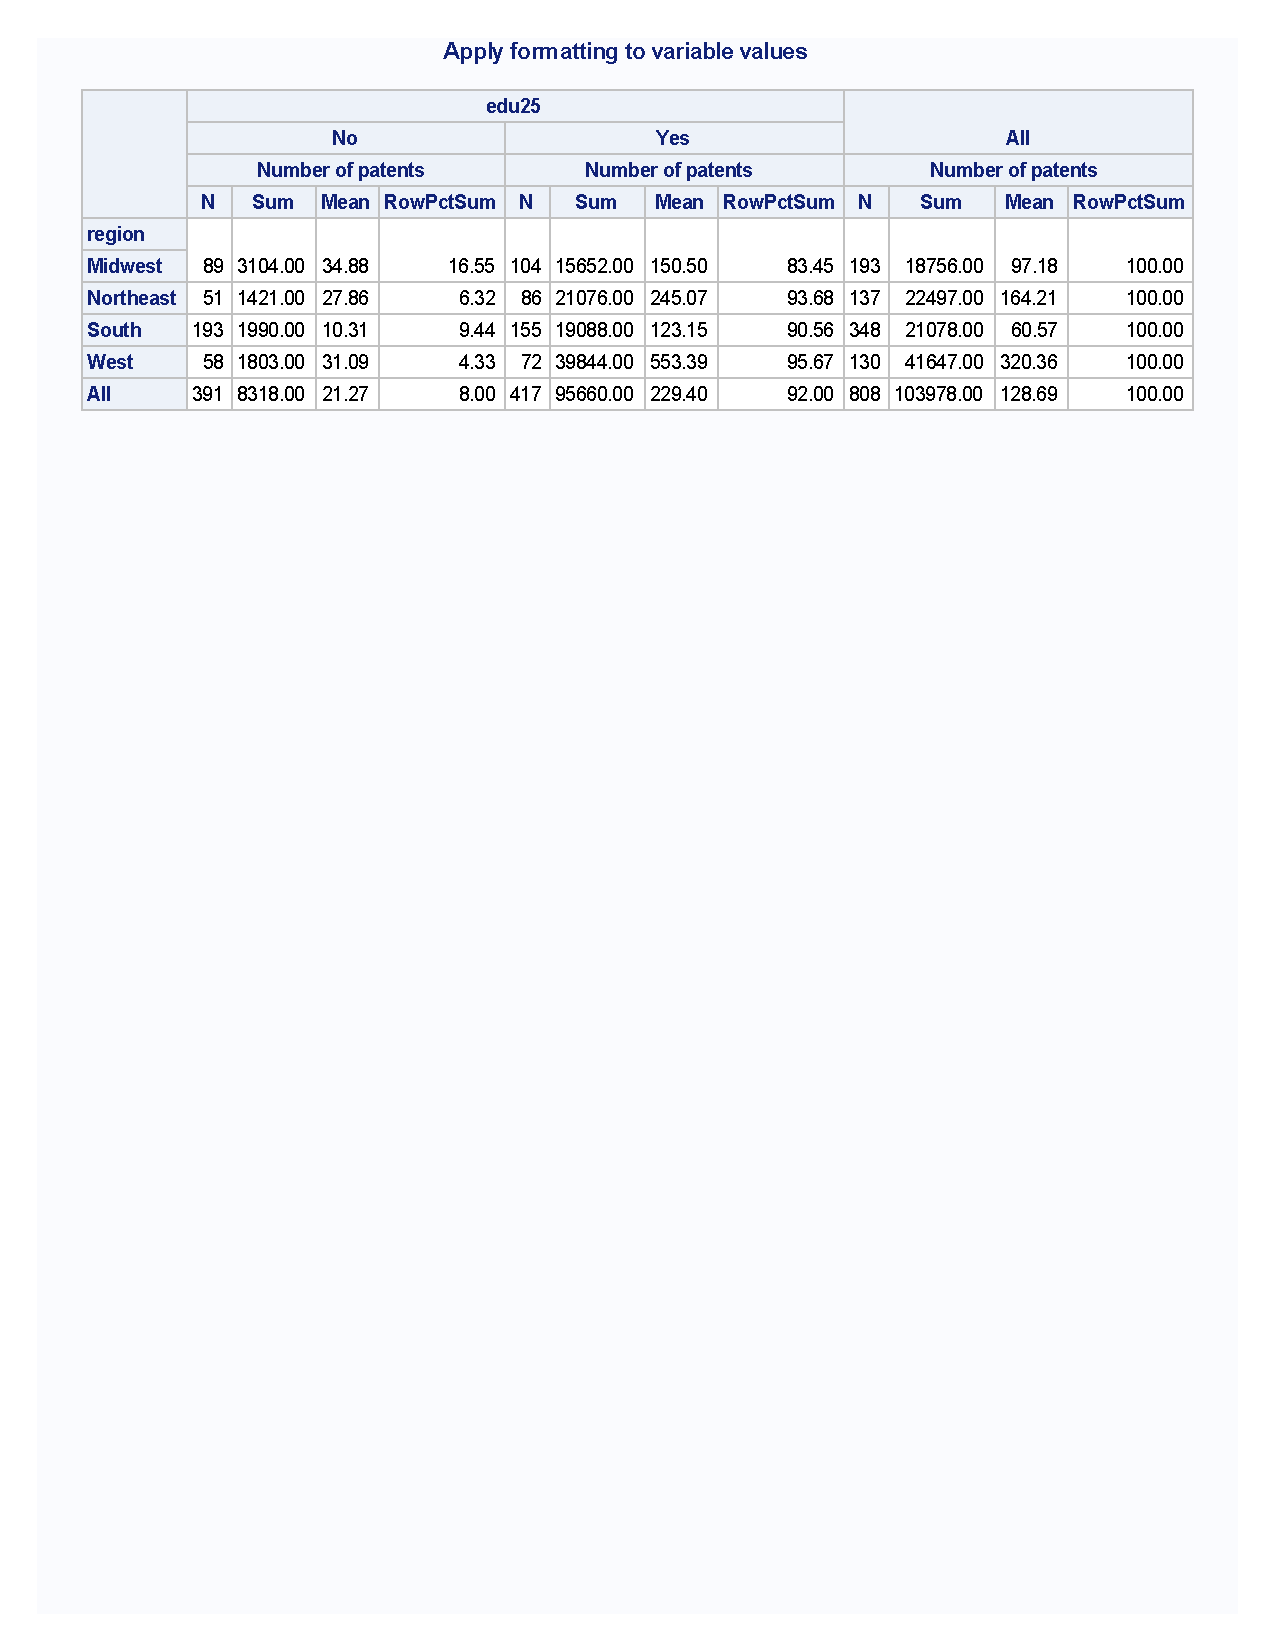
\includegraphics[trim={1cm 20cm 1cm 1.5cm},clip,width=1.0\textwidth]{L15_formatvariable.pdf}\\
%\bi
%\item formats can be applied to variable values
%\item[] \fbox{\ttt{format \emph{variable} \emph{formatname.};}}
%\item formats can be applied to statistics
%\item[] \fbox{\ttt{\emph{statistic}*f=\emph{formatname.}}}
%\ei
\end{frame}


\begin{frame}[fragile]
\ft{Apply formats to statistics}
\hspace*{-0.3in}
\bmp{1.15\textwidth}
\begin{code}{.}
PROC FORMAT ;  PICTURE pct(ROUND) low-high = `009.9\%';  RUN;
PROC TABULATE DATA = patents ;
   CLASS edu25 region;
   VAR patents;
   TABLE region ALL,
   edu25*patents*(N SUM\textcolor{OrangeRed}{*F=COMMA7.} MEAN\textcolor{OrangeRed}{*F=COMMA5.1} ROWPCTSUM\textcolor{OrangeRed}{*F=PCT.})
   ALL*patents*(N SUM\textcolor{OrangeRed}{*F=COMMA7.} MEAN\textcolor{OrangeRed}{*F=COMMA5.1} ROWPCTSUM\textcolor{OrangeRed}{*F=PCT.});
   FORMAT edu25 yn. ;
RUN;
\end{code}
\emp
\vskip10pt
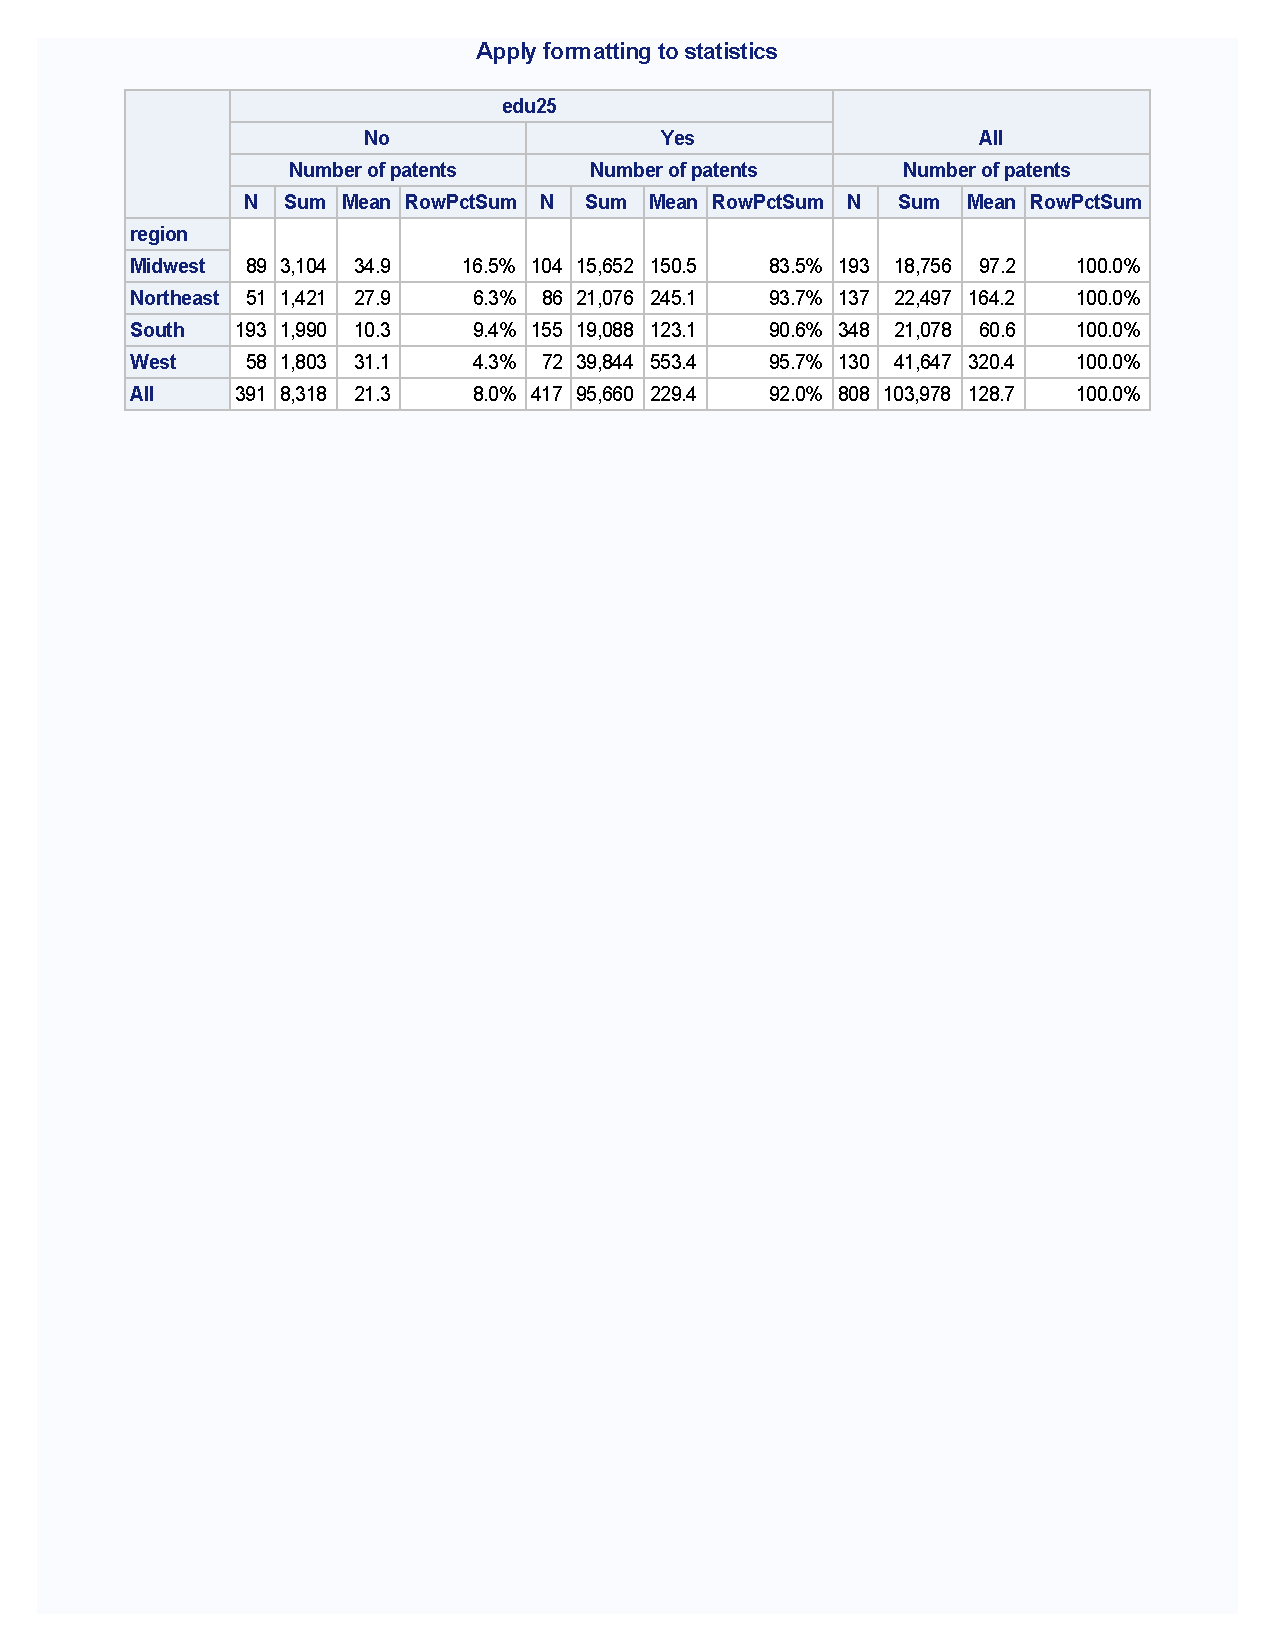
\includegraphics[trim={1cm 20cm 1cm 1.5cm},clip,width=1.0\textwidth]{L15_formatstats.pdf}\\
%\bi
%\item formats can be applied to variable values
%\item[] \fbox{\ttt{format \emph{variable} \emph{formatname.};}}
%\item formats can be applied to statistics
%\item[] \fbox{\ttt{\emph{statistic}*f=\emph{formatname.}}}
%\ei
\end{frame}


\begin{frame}[fragile]
\ft{Basic Labels}
\bmp{1.0\textwidth}
\begin{code}{.}
PROC TABULATE DATA = patents;
   CLASS edu25 region ;
   VAR patents;
   TABLE region\textcolor{OrangeRed}{=" "}  ALL,
     edu25*patents\textcolor{OrangeRed}{=" "}*(N SUM MEAN ROWPCTSUM)
     ALL*patent\textcolor{OrangeRed}{s=" "}*(N SUM MEAN ROWPCTSUM) ;
   \textcolor{OrangeRed}{LABEL edu25="At least 25\% of county has a Bachelor's";}
RUN;
\end{code}
\emp
\vskip10pt
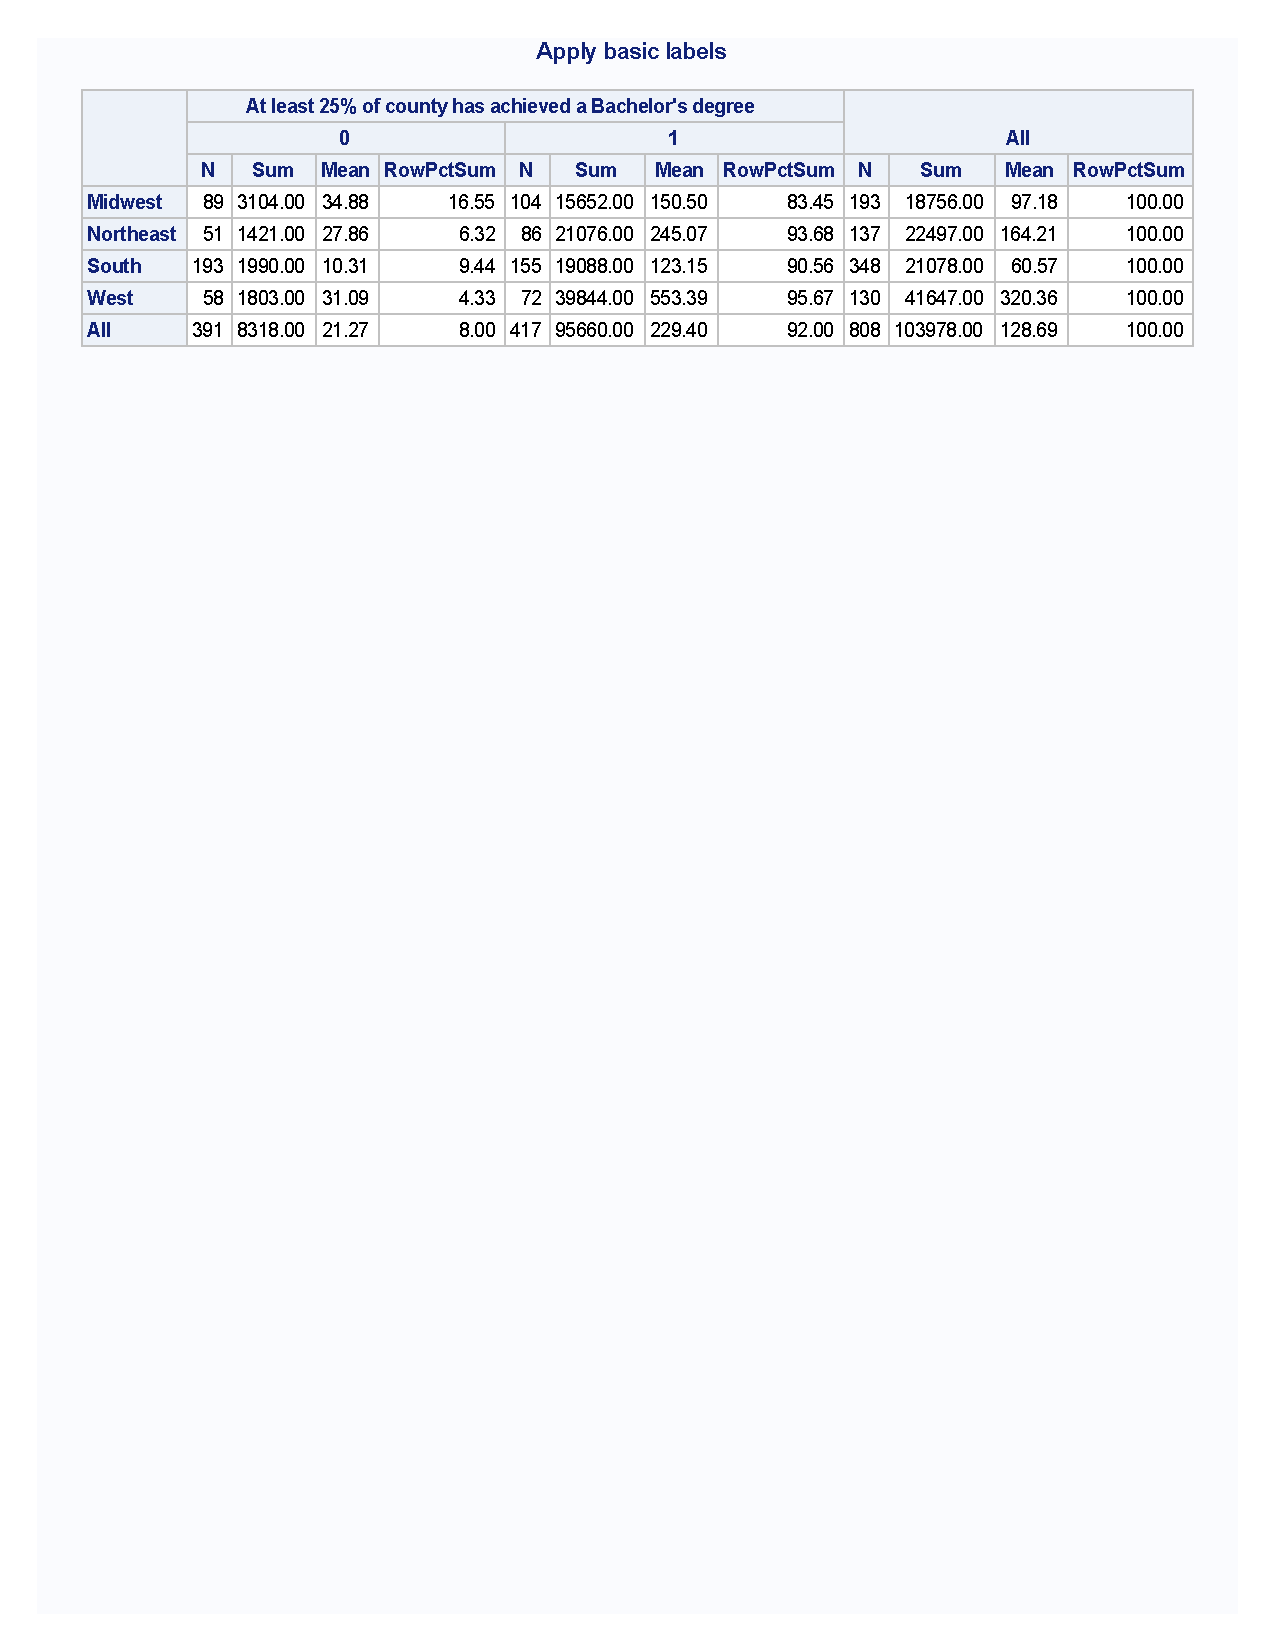
\includegraphics[trim={1cm 20cm 1cm 1.5cm},clip,width=1.0\textwidth]{L15_labels.pdf}\\
%\bi
%\item labels can be applied to variable names two ways
%\item[] \fbox{\ttt{label \emph{variable}=\emph{"Variable Label"};}}
%\item[] \fbox{\ttt{table \emph{variable}=\emph{"Variable Label"};}}
%\item an equal sign with empty label (`` '') removes the cell from the table
%\ei
\end{frame}

\begin{frame}[fragile]
\ft{KeyLabel and Box}
\bmp{1.0\textwidth}
\begin{code}{.}
PROC TABULATE DATA = patents;
   CLASS edu25 region ;
   VAR patents;
   TABLE region=" "  ALL,
         edu25*patents=" "*(N SUM MEAN ROWPCTSUM)
         ALL*patents=" "*(N SUM MEAN ROWPCTSUM) /
         \textcolor{OrangeRed}{BOX = "Geographic Region"};
   LABEL edu25="At least 25\% of county has a Bachelor's";
   \textcolor{OrangeRed}{KEYLABEL ALL="Total" ROWPCTSUM="Row Sum" ;}
RUN;
\end{code}
\emp
\vskip10pt
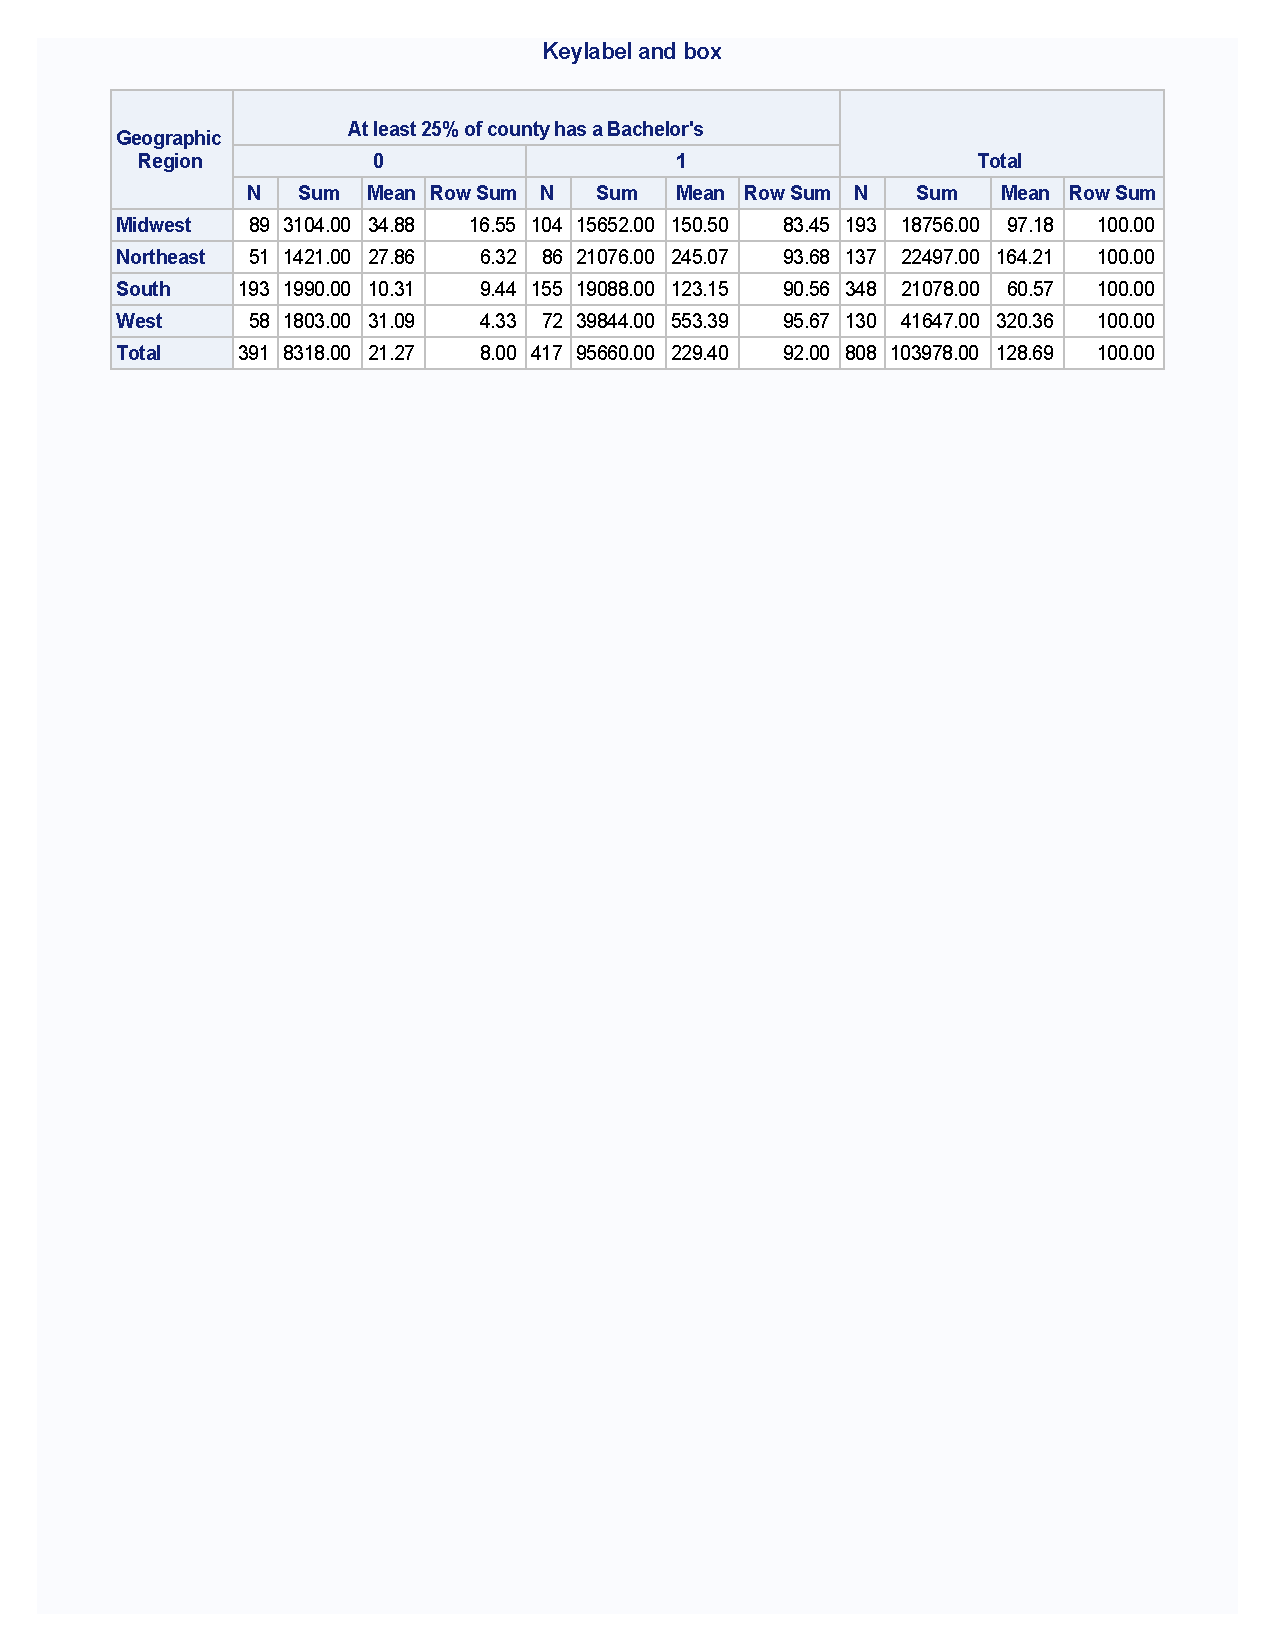
\includegraphics[trim={1cm 20cm 1cm 1.5cm},clip,width=1.0\textwidth]{L15_keybox.pdf}\\

%\bi
%\item \ttt{BOX=} is an \emph{option} in the \ttt{TABLE} statement that changes text in upper left box
%\item \ttt{KEYLABEL} is a statement that applies a label to a \emph{keyword} everywhere that \emph{keyword} appears
%\ei
\end{frame}

\begin{frame}
\ft{Cell colors}
\bi
\item
To apply a background color to all cells, use the following in a \ttt{TABLE} statement:
\fbox{\ttt{\emph{variable}*\{STYLE=\{BACKGROUND=\emph{mycolor}\}\}}}
%\item[] \emph{mycolor} does \underline{not} go in quotes
\item
To highlight individual cells based on their values (trafficlighting)
\begin{enumerate}
\item Create a format that specifies color based on values
\item[] \fbox{\ttt{PROC FORMAT; VALUE \emph{myhl} 95-high="\emph{mycolor}"; RUN;}}
%\item[] \emph{mycolor} \underline{does} go in quotes
\item Apply the format to the background style in the \ttt{TABLE} statement
\item[]
\fbox{\ttt{\emph{statistic}*\{STYLE=\{BACKGROUND=\emph{myhl.}\}\}}}
\end{enumerate}
\item
Predefined SAS colors: \url{http://support.sas.com/documentation/cdl/en/graphref/67881/HTML/default/viewer.htm\#n161ukdyz9wpfsn1nh8sihforvyq.htm}
\ei
\end{frame}

\begin{frame}[fragile]
\ft{Highlight cells}
\hspace{-0.3in}
\bmp{1.15\textwidth}
\begin{code}{.}
PROC FORMAT ;  VALUE hlpct 95-high="Chartreuse" ; RUN ;
PROC TABULATE DATA=patents;
CLASS region; 
CLASS edu25 / DESCENDING;
VAR patents;
TABLE region=" "  ALL,
edu25*patents=" "*
  (N SUM*F=COMMA7. 
   MEAN*F=COMMA5.1 
   ROWPCTSUM*F=PCT.\textcolor{OrangeRed}{*\{STYLE=\{BACKGROUND=HLPCT.\}\}})
ALL*patents=" "*
  (N SUM*F=COMMA7. MEAN*F=COMMA5.1 ROWPCTSUM*F=PCT.) /
BOX="Geographic Region";
LABEL edu25="At least 25\% of county has a Bachelor's";
KEYLABEL ALL="Total" ROWPCTSUM="Row Sum" ; 
FORMAT edu25 yn.;
RUN;
\end{code}
\emp
%\bi
%\item \ttt{BOX=} is an \emph{option} in the \ttt{TABLE} statement that changes text in upper left box
%\item \ttt{KEYLABEL} is a statement that applies a label to a \emph{keyword} everywhere that \emph{keyword} appears
%\ei
\end{frame}

\begin{frame}[fragile]
\ft{Final table}
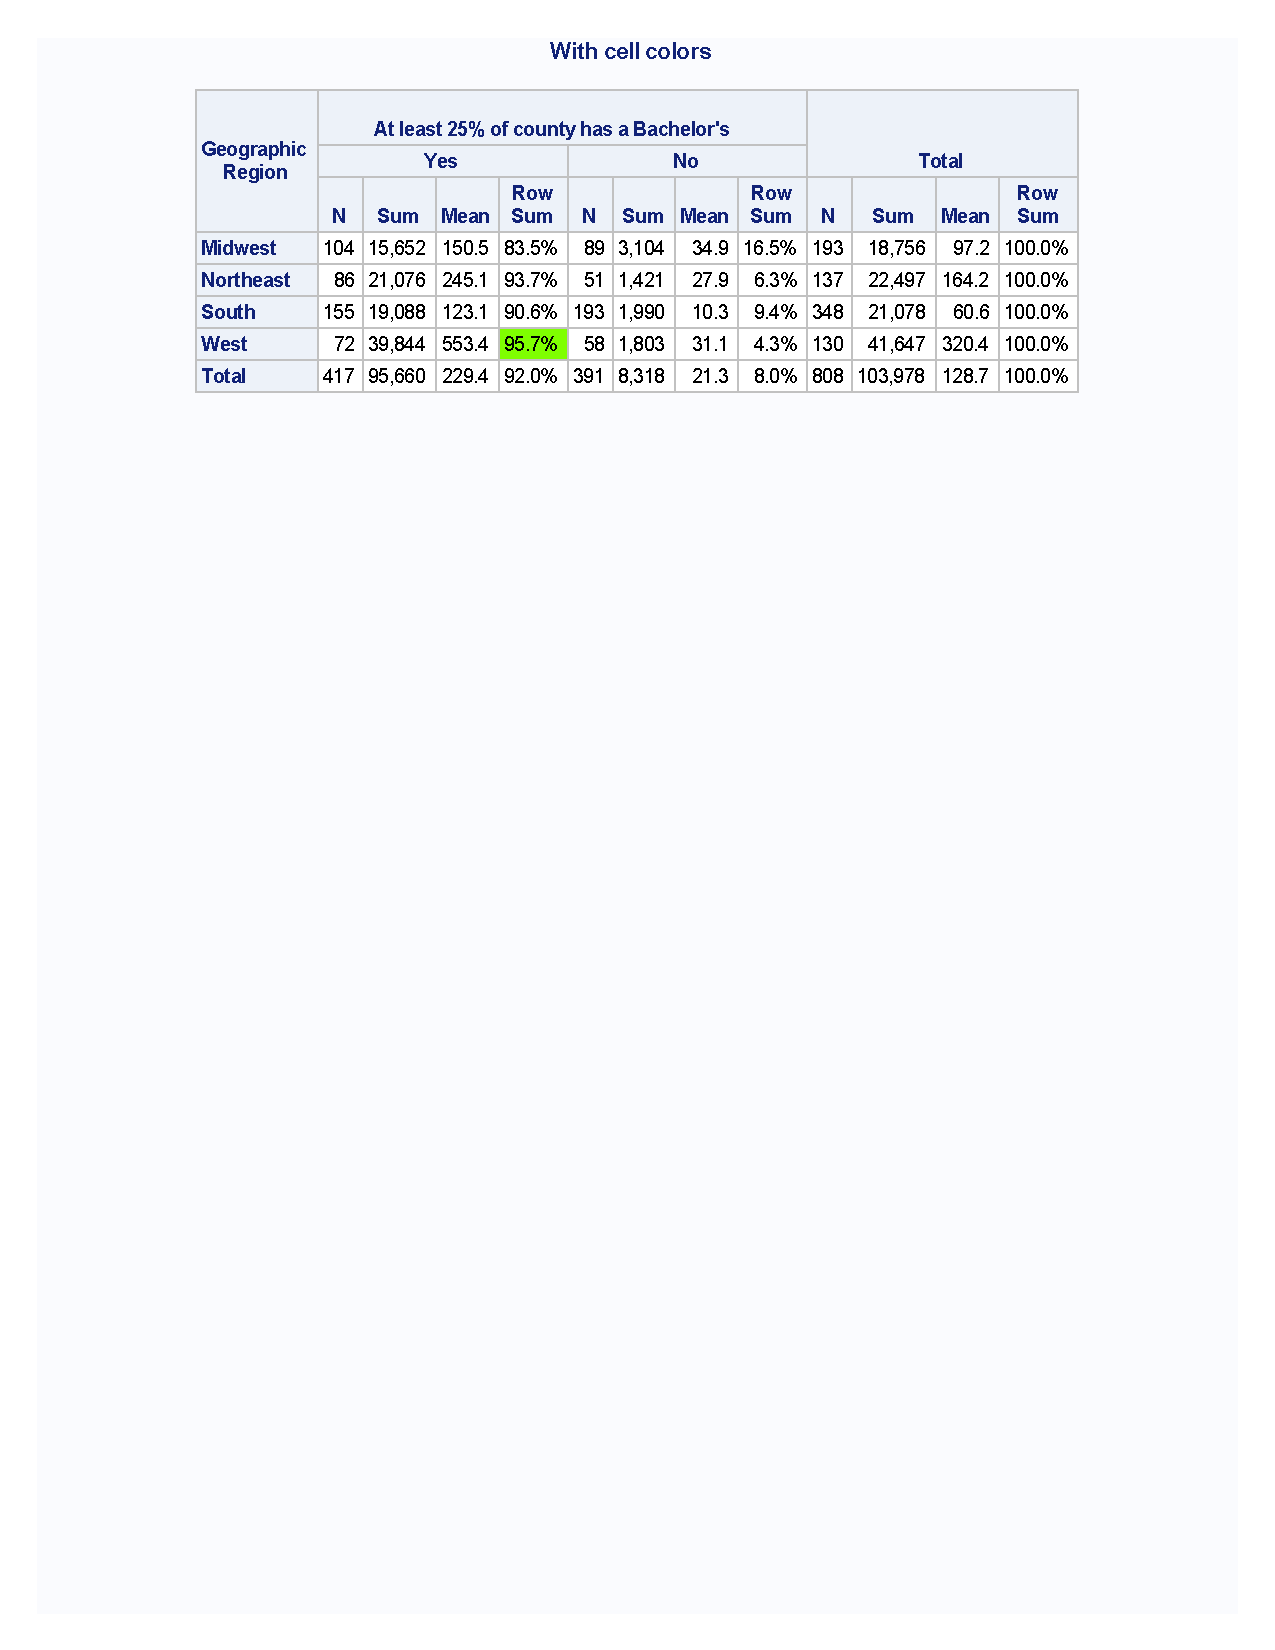
\includegraphics[trim={1cm 20cm 1cm 1.5cm},clip,width=1.0\textwidth]{L15_highlight.pdf}
\end{frame}
%
%\begin{frame}[fragile]
%\ft{Using ODS to export your table}
%\bmp{1.0\textwidth}
%\begin{code}{.}
%ods pdf file="/Computer Path/\emph{TableName}.pdf" style=\emph{mystyle};
%   proc tabulate data=patents; ... run;
%ods pdf close;
%
%ods rtf file="/Computer Path/\emph{TableName}.rtf" style=\emph{mystyle};
%    proc tabulate data=patents; ... run;
%ods rtf close;
%\end{code}
%\emp
%\bi
%\item[]
%\item \ttt{rtf} can be useful for inserting into word docs
%\item style options: \url{http://www.stattutorials.com/SAS/Tutorial_SAS_ODS_Styles.htm}
%\ei
%\end{frame}



\end{document} 